\chapter{FUNDAMENTAÇÃO TEÓRICA}\label{CAP4}
Nesta seção serão abordados todos os assuntos que foram estudados para a contrução deste trabalho.
\section{SISTEMAS E SOFTWARE EMBARCADOS}\label{secaosistemasembarcados}
A definição de sistemas embarcados, segundo \citeonline{leeseshia}, são sistemas computacionais pouco perceptíveis, que geralmente são responsáveis por executar pequenas atividades de forma autônoma, como controlar os robôs da linha de produção de uma fábrica ou gerenciar os semáforos de uma cidade. De acordo com \citeonline{carrowagner} os sistemas computacionais embarcados estão presentes em boa parte das atividades humanas, passando desde o sistema de transporte até os eletrodomésticos de uma residência. Baseado nestes argumentos, sistemas embarcados são todos os dispositivos com poder de processamento, memória e fontes de energia limitados \cite{leeseshia}, que podem se integrar com o meio físico.

\citeonline{leeseshia} ainda reforçam que os programas que são executados nestes dispositivos são chamados de software embarcado. \apudonline{gill}{leeseshia} da \textit{National Science Foundation in the US} cria o termo sistemas ciberfísicos \textit{(Cyber-Physical Systems – CPS)} para se referir à integração da computação com processos físicos. Observa-se aqui uma outra definição para sistemas embarcados. No \textit{CPS}, os sistemas informatizados monitoram e controlam os processos físicos geralmente executando instruções dentro de loops. \citeonline{leeseshia} ainda reforça que é importante compreender a dinâmica dos sistemas computacionais junto com os processos físicos. Por lidar diretamente com o mundo físico, o tempo necessário para executar uma tarefa, nos sistemas ciberfísicos, pode ser fundamental para o correto funcionamento do sistema. A passagem do tempo no mundo físico é algo crítico, ao contrário do mundo cibernético.

Enquanto no processo físico existem diversas coisas acontecendo concorrentemente (ao mesmo tempo), nos processos de software as atividades acontecem em etapas sequenciais. \citeonline{leeseshia} afirmam que o maior desafio técnico na concepção e análise do software embarcado se deriva da necessidade de unir a semântica sequencial do mundo lógico com a realidade concorrente do mundo físico.

\section{SISTEMAS DISTRIBUÍDOS}\label{secaosistemasdistribuidos}
Um sistema distribuído, segundo \citeonline{tanenbaum}, é um conjunto de computadores independentes que que se apresentam ao usuário final como um único sistema coerente. De maneira genérica, a arquitetura de um sistema distribuído é composto por diversos itens de hardware que atuam de forma autônoma - geralmente processando informações específicas - mas que se comunicam entre si caracterizando-se como apenas um único hardware responsável pelo sistema como um todo. O autor ainda reforça que as pessoas ou usuários acham que estão interagindo com um sistema apenas, e não com um conjunto de sistemas. Contudo, para garantir a operação de todo este conjunto, é preciso que haja a colaboração de todos os componentes e dispositivos que fazem parte do sistema. A essência do sistema distribuído está em estabelecer essa colaboração.

Não é estabelecido nenhum padrão ou premissa relacionado ao tipo de hardware que irá compor o sistema. \citeonline{tanenbaum} ainda afirma que esses dispositivos podem variar desde computadores centrais até pequenos nós em redes de sensores. Também não existe premissa com relação ao modo com que os dispositivos se interligam. A característica principal dos sistemas distribuídos está em ocultar boa parte da comunicação interna deste conjunto ao usuário. \citeonline{tanenbaum} define ainda quatro metas que devem ser cumpridas para que o esforço necessário para a construção de um sistema distribuído seja válida: o sistema deve oferecer fácil acesso a seus recursos; deve ocultar razoavelmente bem o fato de que os recursos são distribuídos por uma rede; deve ser aberto e deve permitir a sua expansão.

\section{ARQUITETURA DO SISTEMA AUTOMOTIVO}
Para compreender como funciona a comunicação interna do veículo, é necessário antes saber como o sistema está estruturado, quais dispositivos e controladores utilizados, qual a arquitetura adotada e quais protocolos estão implementados. Para \citeonline{navetsimonotlion}, os fabricantes de automóveis diferenciam em várias categorias os eletrônicos embarcados que um carro possui. Eles utilizam essas categorias para agrupar sistemas mecânicos e ou eletrônicos de acordo com as suas funcionalidades.

\subsection{\textbf{Categorias funcionais dos sistemas embarcados automotivos}}
Historicamente, segundo os autores, existem cinco categorias de sistemas embarcados: \textit{Power Train}, \textit{Chassis}, \textit{Body}, \textit{HMI} e \textit{Telematics}. A categoria \textit{Power Train} fazem parte todos os sistemas que participam da propulsão longitudinal do veículo, incluindo o motor, a transmissão e todos os componentes que dão apoio para esta função. A categoria \textit{Chassis} se refere às quatro rodas e à sua posição relativa de movimento. Nesta categoria os principais sistemas são o de freios e direção. Dentro da categoria \textit{Body} estão presentes as entidades que não pertencem à dinâmica do veículo, mas que auxiliam o motorista, como o airbag, limpadores, iluminação, vidros, ar condicionado, assentos, etc. Já a categoria \textit{HMI} inclui o equipamento que permite a troca de informações entre os sistemas eletrônicos e o motorista do veículo. Por fim, a categoria \textit{Telematics} está relacionado à componentes que permitem a troca de informações do veículo com o mundo exterior, como rádio, sistemas de navegação, GPS, entre outros. \citeonline{navetsimonotlion} ainda ressaltam que cada categoria do sistema eletrônico possui características bem diferentes, o que faz com que cada dispositivo tenha um requisito ou uma restrição bem definida. A Figura \ref{Fig:categorias_sistemas_embarcados} ilustra a divisão funcional dos sistemas pelas categorias.

\begin{figure}[!ht]
\centering
\caption{Representação das cinco categorias funcionais.} 
{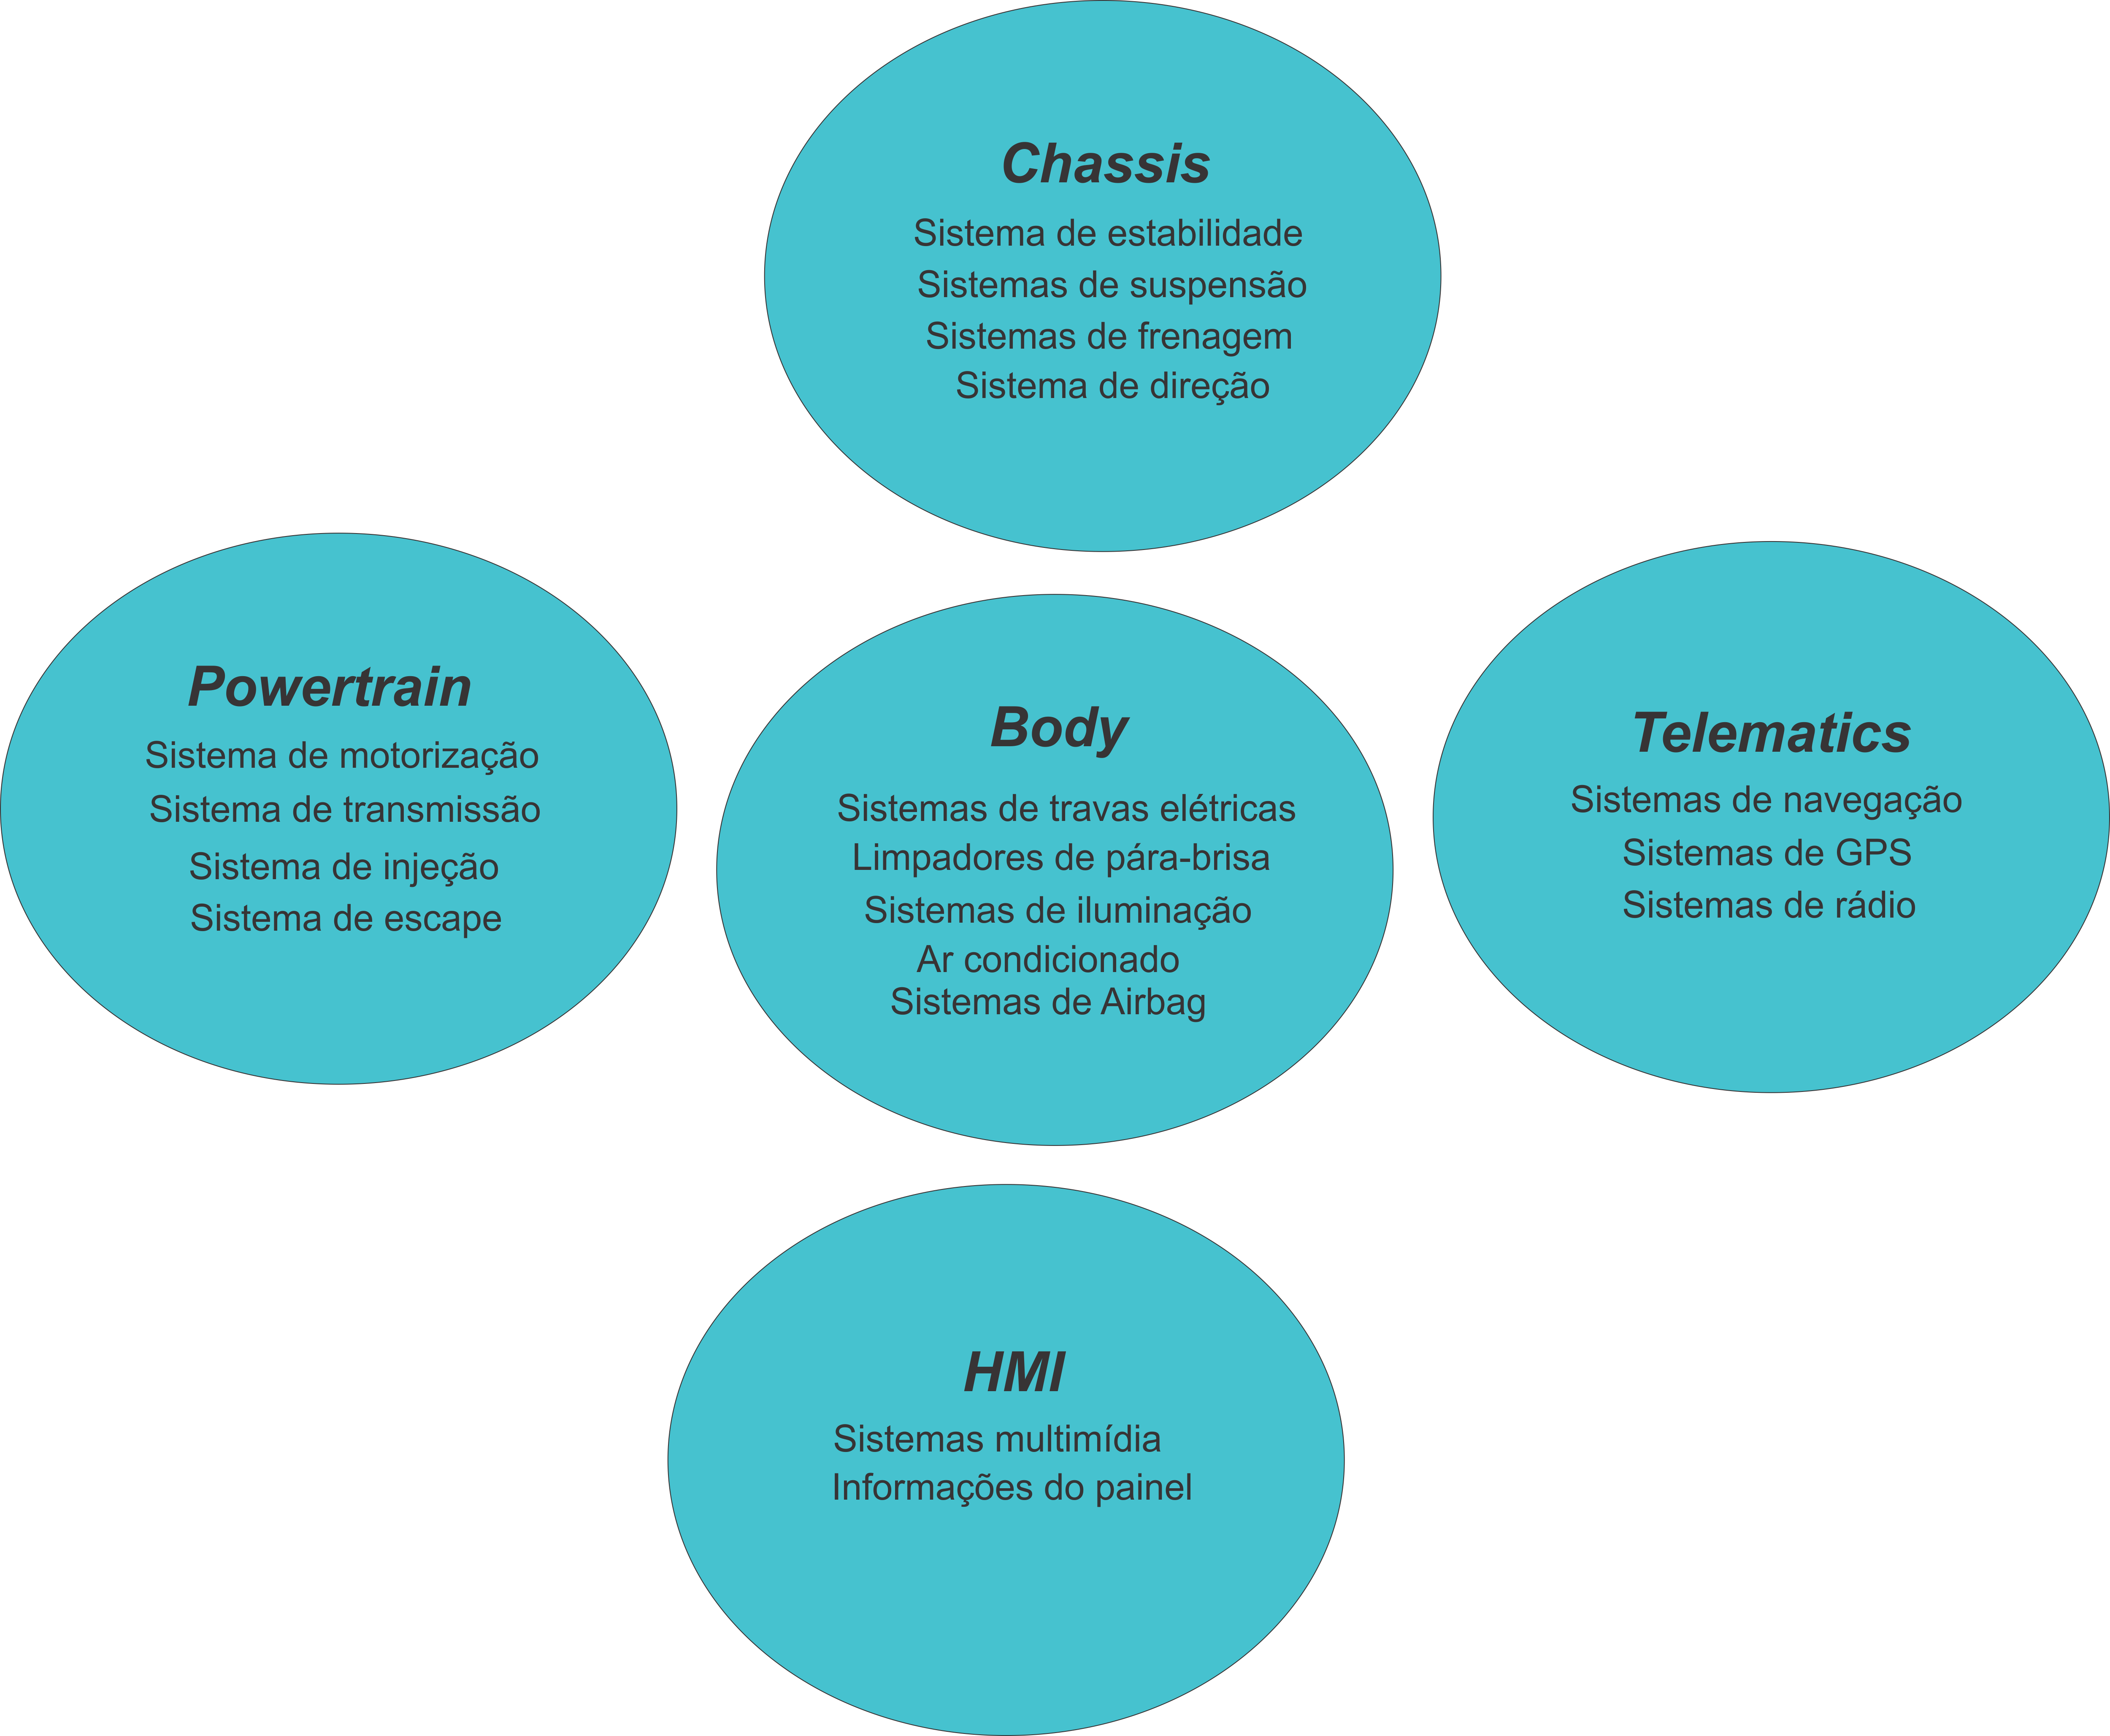
\includegraphics[scale=.31]{imagens/categoriaFuncionalSistemasEmbarcados.png}}\\
\makebox[\width]{Fonte: baseado em \citeonline{navetsimonotlion}} \label{Fig:categorias_sistemas_embarcados}
\end{figure}


\begin{itemize}
\item{Categoria \textit{Power Train}:}
Além de controlar a velocidade do motor, atuando de acordo com as intervenções do motorista no pedal, o controlador pode também, atuar de acordo com fatores naturais, como a temperatura do ar ou o nível de oxigênio, ou atuar de acordo com os distúrbios ambientais, como a poluição dos gases de escape ou o ruído. Ainda segundo \citeonline{navetsimonotlion}, o controlador é projetado para otimizar alguns parâmetros. O parâmetro mais comum a ser controlado é a quantidade de combustível que deve ser injetado para combustão de acordo com a rotação do motor e a posição do pedal do acelerador. Observa-se que nesta categoria estão presentes todos os dispositivos que auxiliam no gerenciamento do motor, tanto de forma direta quanto indireta.

\item{Categoria \textit{Chassis}:}
Nesta categoria, existem sistemas responsáveis por gerenciar a interação do veículo com a estrada. O objetivo destes sistemas é controlar o automóvel de acordo com as solicitações do motorista, como frenagem ou aceleração, considerando também o perfil da via ou as condições ambientais, visando sempre o conforto e a segurança dos passageiros. \citeonline{navetsimonotlion} ainda reforça que esses sistemas devem ser de alta qualidade, como qualquer sistema crítico. Os sistemas mais comuns são o de frenagem (ABS) e o controle automático de estabilidade (ASC).

\item{Categoria \textit{Body}:}
Limpadores de para-brisa, luzes, portas e janelas e outros itens são controlados por sistemas pertencentes a esta categoria. Estes, por sua vez, não estão sujeitos a restrições de desempenho rigorosas, e do pondo de vista de segurança, segundo os autores, não representam uma parte crítica do sistema. Entretanto, existem certas funções, como controlar o acesso ao veículo, que deve respeitar as dificuldades em tempo real.

\item{Categoria \textit{HMI}:}
Os sistemas presentes nesta categoria, em geral, permite a interação do motorista com diversas funções integradas no veículo. Uma das funções é exibir o estado atual do veículo, como velocidade, rotação do motor e temperatura, por exemplo, ou também mostrar o estado de algum dispositivo multimídia.

\item{Categoria \textit{Telematics}:}
Esta categoria, ainda segundo \citeonline{navetsimonotlion}, inclui sistemas que suportam trocas de informações entre infra-estruturas viárias e rodoviárias. Um exemplo está relacionado com a cobrança automática de pedágios. Para os autores, em um futuro próximo, esta categoria permitirá otimizar o uso rodoviário através da gestão do tráfego a fim de evitar congestionamentos.
\end{itemize}

A divisão dos sistemas por categoria engloba dispositivos de acordo com suas semelhanças funcionais. Logo, se um conjunto eletrônico, mesmo que sejam diferentes, seguirem um determinado requisito comum à uma categoria, estes pertencerão à esta. Entretanto, os sistemas eletrônicos, mesmo pertencendo à uma categoria distinta, não são impedidos de se comunicarem entre si. Segundo o exemplo de \citeonline{navetsimonotlion}, as informações como a rotação do motor, temperatura ou a velocidade fazem parte do gerenciamento do motor, e logo pertencem à categoria \textit{power train}, mas são transmitidas desta para a categoria \textit{HMI}, para exibir as informações do veículo ao motorista no painel de instruções (Figura \ref{Fig:comunicacao_categorias_sistemas_embarcados}).

\begin{figure}[!ht]
\centering
\caption{Representação do monitoramento de RPM e a comunicação entre as categorias.} 
{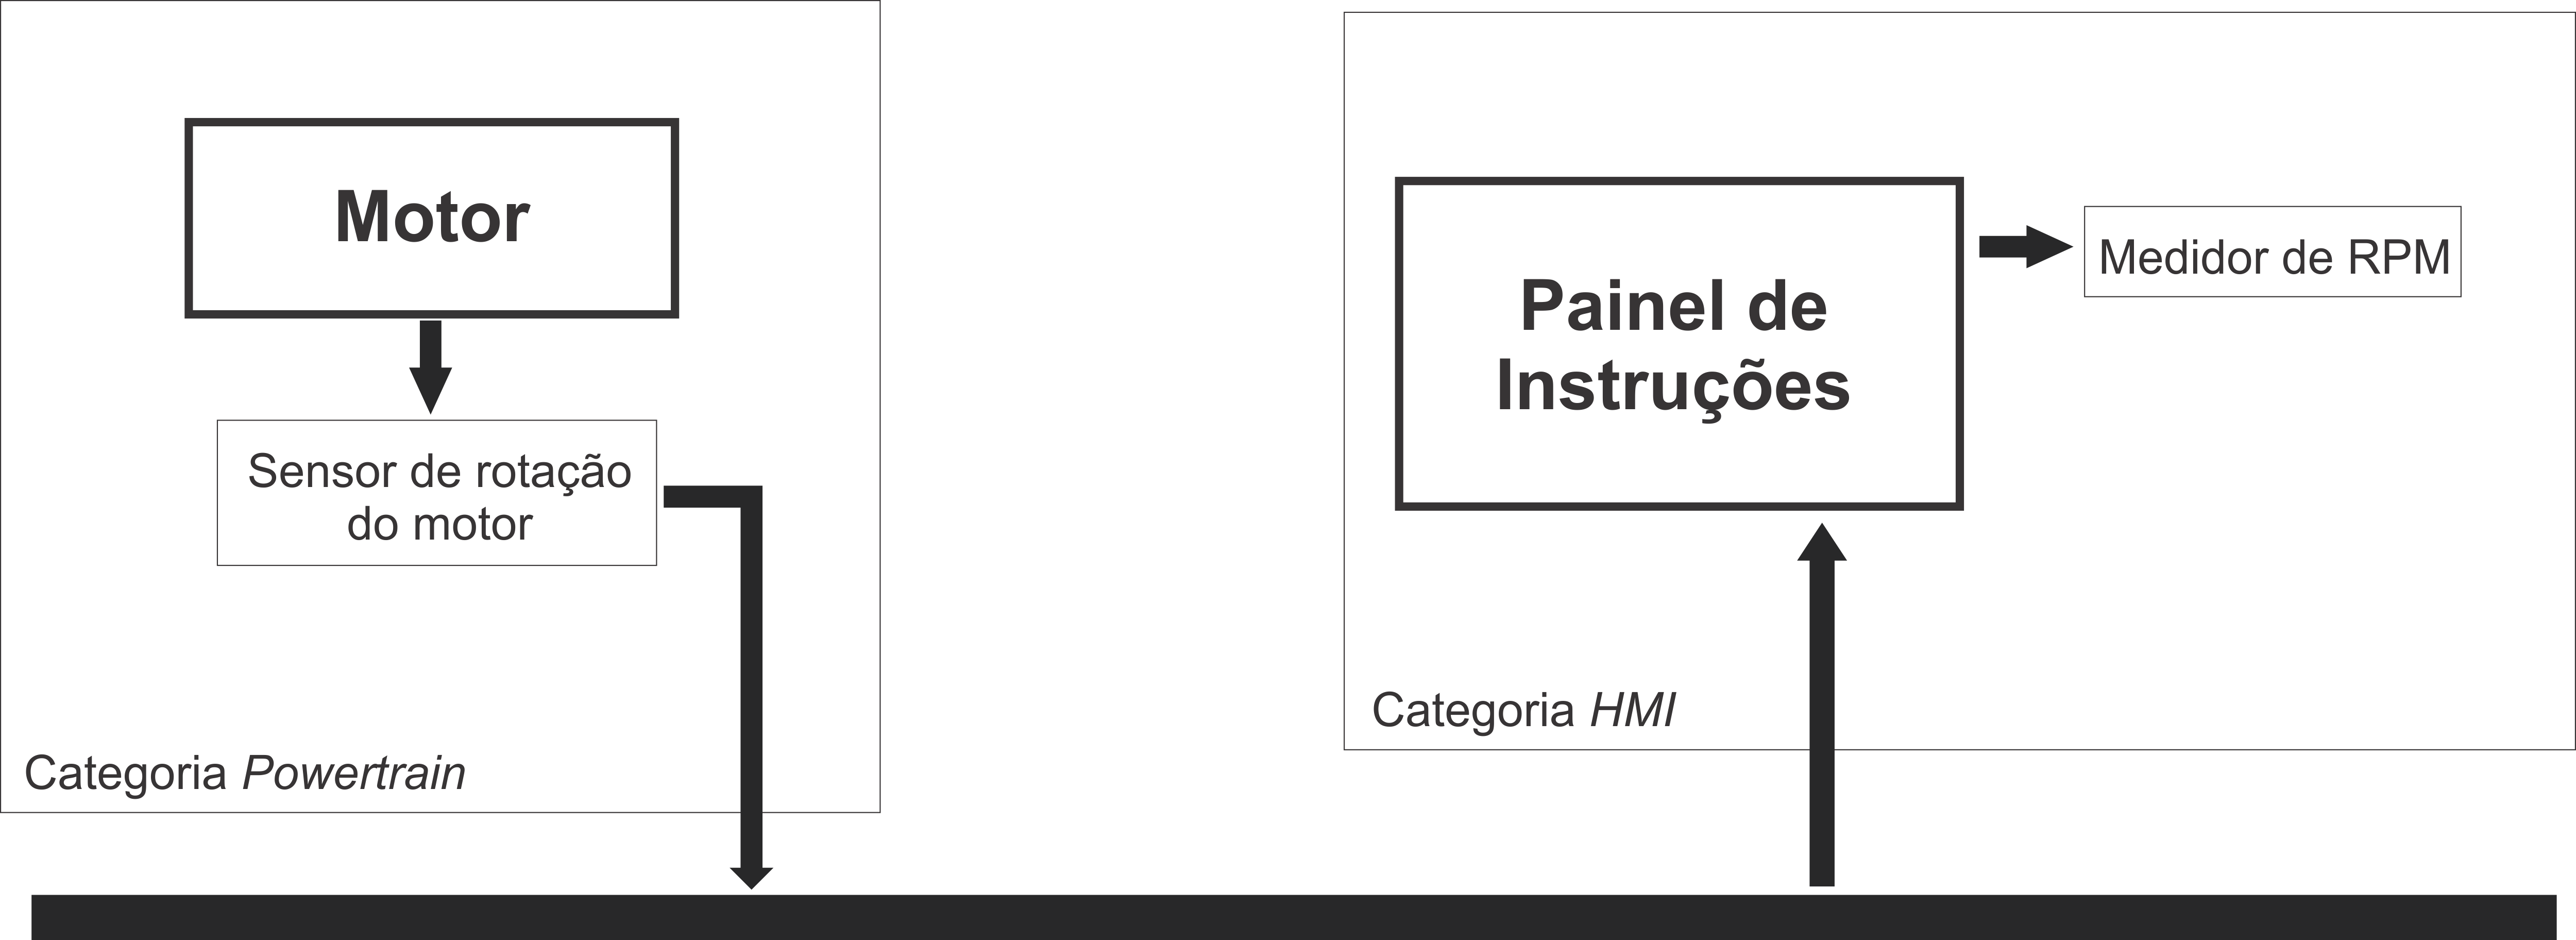
\includegraphics[scale=.37]{imagens/intercomunicacaoEntreCategorias.png}}\\
\makebox[\width]{Fonte: baseado em \citeonline{navetsimonotlion}} \label{Fig:comunicacao_categorias_sistemas_embarcados}
\end{figure}

Analisando o funcionamento destes sistemas eletrônicos, eles são caracterizados como sistemas embarcados automotivos pelo fato de possuírem uma forte interação com o mundo físico, conforme a definição de sistemas embarcados explorado na seção \ref{secaosistemasembarcados}. Para interagir com o mundo físico, estes sistemas fazem o uso de outros dispositivos conhecidos como sensores e atuadores. Segundo \citeonline{leeseshia}, um sensor mede uma quantidade física, enquanto o atuador altera a quantidade física. Eles ainda complementam que estes dispositivos conectam o mundo cibernético com o mundo físico. Em outras palavras, um sensor obtém os dados de uma leitura, e o atuador realiza uma ação que foi passado a ele. Em um automóvel existem diversos sensores espalhados por sua estrutura e que monitoram diversos aspectos físicos do veículo, como aceleração lateral, velocidade e tração individual das rodas, monitorando a estabilidade do carro durante o percurso \cite{navetsimonotlion}. O autor ainda complementa que quando uma correção precisa ser aplicada nesta situação, as rodas dianteiras ou traseiras podem frear individualmente e com intensidades diferentes, ou atuar na redução da potência do motor. Percebe-se neste exemplo a ação dos atuadores no meio físico. A Figura \ref{Fig:relacao_sensor_atuador} representa a influência destes dispositivos no meio físico.

\begin{figure}[!ht]
\centering
\caption{Representação da atuação dos sensores e atuadores.} 
{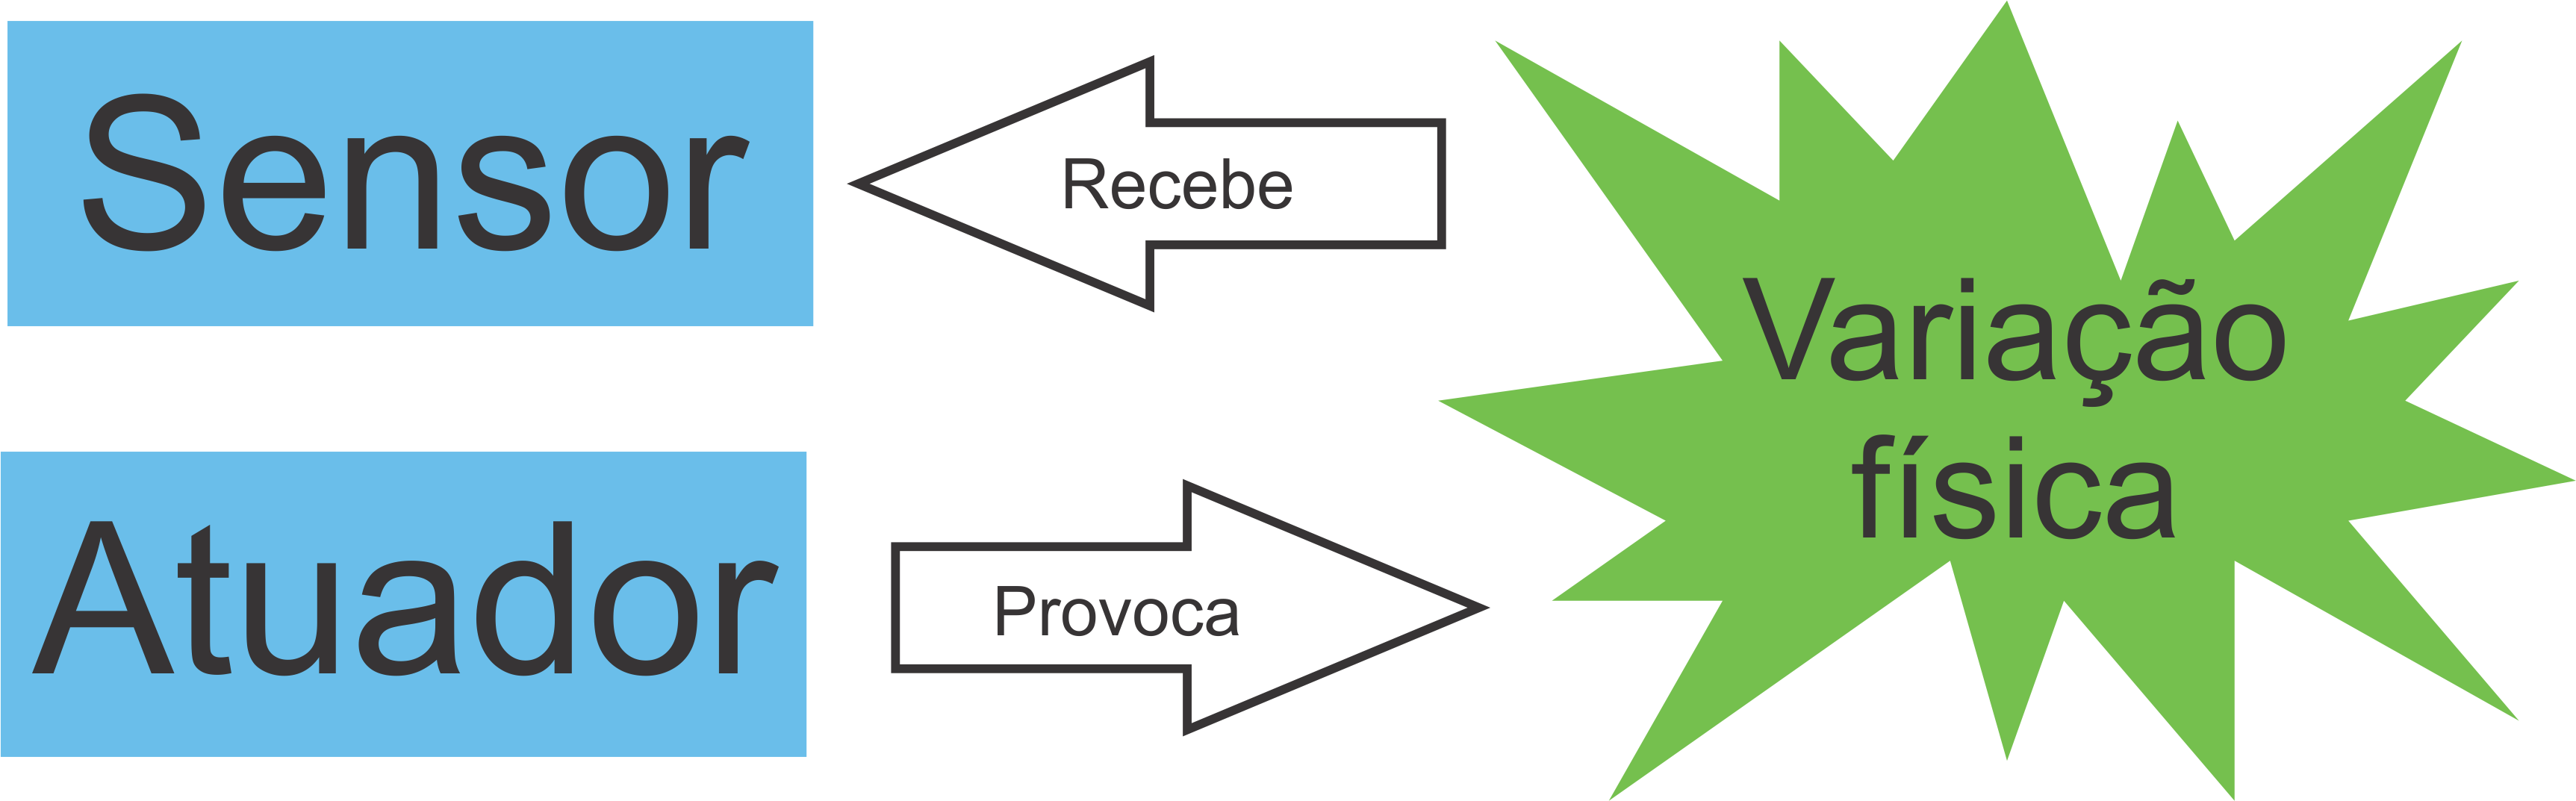
\includegraphics[scale=.29]{imagens/relacaoSensorAtuador.png}}\\
\makebox[\width]{Fonte: baseado em \citeonline{leeseshia}} \label{Fig:relacao_sensor_atuador}
\end{figure}

Analisando-se também a forma como esses dispositivos trocam informações uns com os outros, percebe-se que está presente o conceito de sistemas distribuídos, conforme apresentado na seção \ref{secaosistemasdistribuidos}. Um exemplo desse conceito no cenário automotivo é mencionado por \citeonline{navetsimonotlion}, que está relacionado com a funcionalidade de piloto automático \textit{(cruise control)} presente em alguns modelos de veículos. Para que esse sistema funcione perfeitamente, segundo os autores, é necessário a troca de dados de vários sensores que podem pertencer a categorias funcionais distintas. A função de piloto automático tem a responsabilidade central de processar esses dados vindos de diversas origens e enviar as respostas a vários outros dispositivos de saída para cumprir seu objetivo.

Desde a década de 70, como aponta \citeonline{navetsimonotlion}, houve um aumento muito grande no número de sistemas que passaram a substituir os que eram puramente mecânicos ou hidráulicos. O desempenho e confiabilidade desses componentes de hardware que passaram a integrar o automóvel permite a execução de funções complexas, aumentando o conforto e a segurança dos ocupantes do veículo. A arquitetura de hardware de um automóvel não é composta somente de sensores, atuadores, controladores e links de comunicação que permite a interconexão dos componentes, mas também de dispositivos conhecidos como \textit{ECUs}.

\subsection{\textbf{\textit{ECU (Eletronic Control Unit)}}}
Um veículo possui alguns controladores eletrônicos, que para \citeonline{smith}, são chamados de dispositivos informatizados que passam por diversos nomes diferentes, como Unidade de Controle Eletrônico \textit{(Eletronic Control Unit - ECU)}, Unidade de Controle do Motor \textit{(Engine Control Unit – ECU)}, Unidade de Controle de Transmissão \textit{(Transmission Control Unit – TCU)} ou ainda Módulo de Controle de Transmissão \textit{(Transmission Control Module – TCM)}. O autor ainda destaca que esses termos na teoria podem ter significados específicos em uma determinada configuração, mas na prática acaba utilizando-se o termo \textit{ECU} que é comum a eles. Isso porque independente do tipo de controlador eletrônico, eles acabam executando as mesmas funções, ou funções extremamente semelhantes. \citeonline{navetsimonotlion} afirmam que um dos principais propósitos dos sistemas eletrônicos é auxiliar o condutor a controlar o veículo. Segundo eles, a \textit{ECU} autônoma é um subsistema composto por um microcontrolador e um conjunto de sensores e atuadores associados. Os autores também trazem a ideia de que as \textit{ECUs} podem aprimorar a ação dos atuadores, indo muito além da capacidade humana sobre eles. A Figura \ref{Fig:ecu} apresenta a foto de uma \textit{ECU}.

\begin{figure}[!ht]
\centering
\caption{Foto de uma \textit{ECU}.} 
{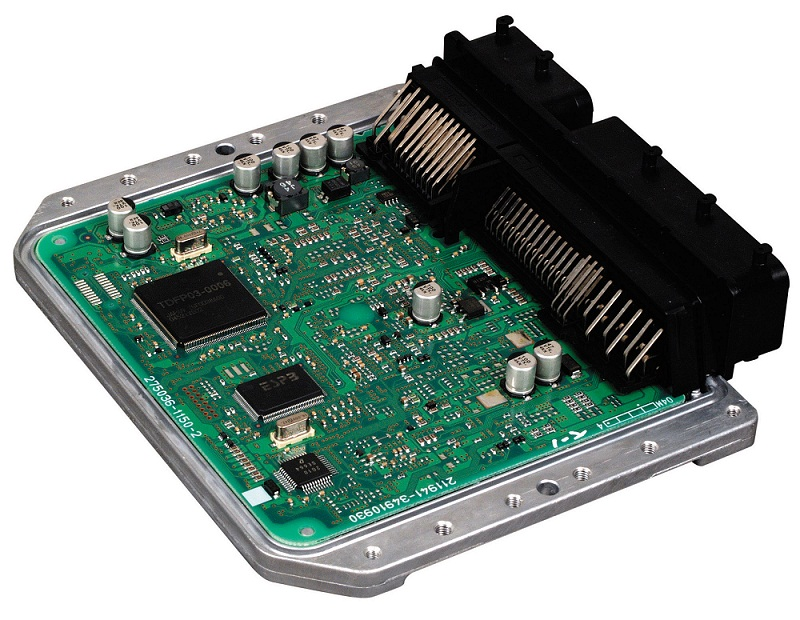
\includegraphics[scale=1.3]{imagens/ecu1.jpg}}\\
\makebox[\width]{Fonte: imagem extraída do artigo de \citeonline{carrosinfoco} do site Carros Infoco} \label{Fig:ecu}
\end{figure}

Em outras palavras, a \textit{ECU}, de forma geral, é um dispositivo capaz de processar as informações recebidas pelos sensores dos veículos, e gerar uma resposta para a ação dos atuadores, conforme está representado na Figura \ref{Fig:relacao_ecu_sensor_atuador}. Como a \textit{ECU} faz parte de um sistema embarcado, sua memória e capacidade de processamento são limitadas assim como qualquer dispositivo embarcado, conforme abordado na seção \ref{secaosistemasembarcados}. Entretanto, as \textit{ECUs} são destinadas a executar determinadas tarefas em específico, de modo que o desempenho do sistema como um todo não seja afetado pela limitação de hardware do dispositivo.

\begin{figure}[!ht]
\centering
\caption{Diagrama da comunicação entre \textit{ECU}, sensor e atuador.} 
{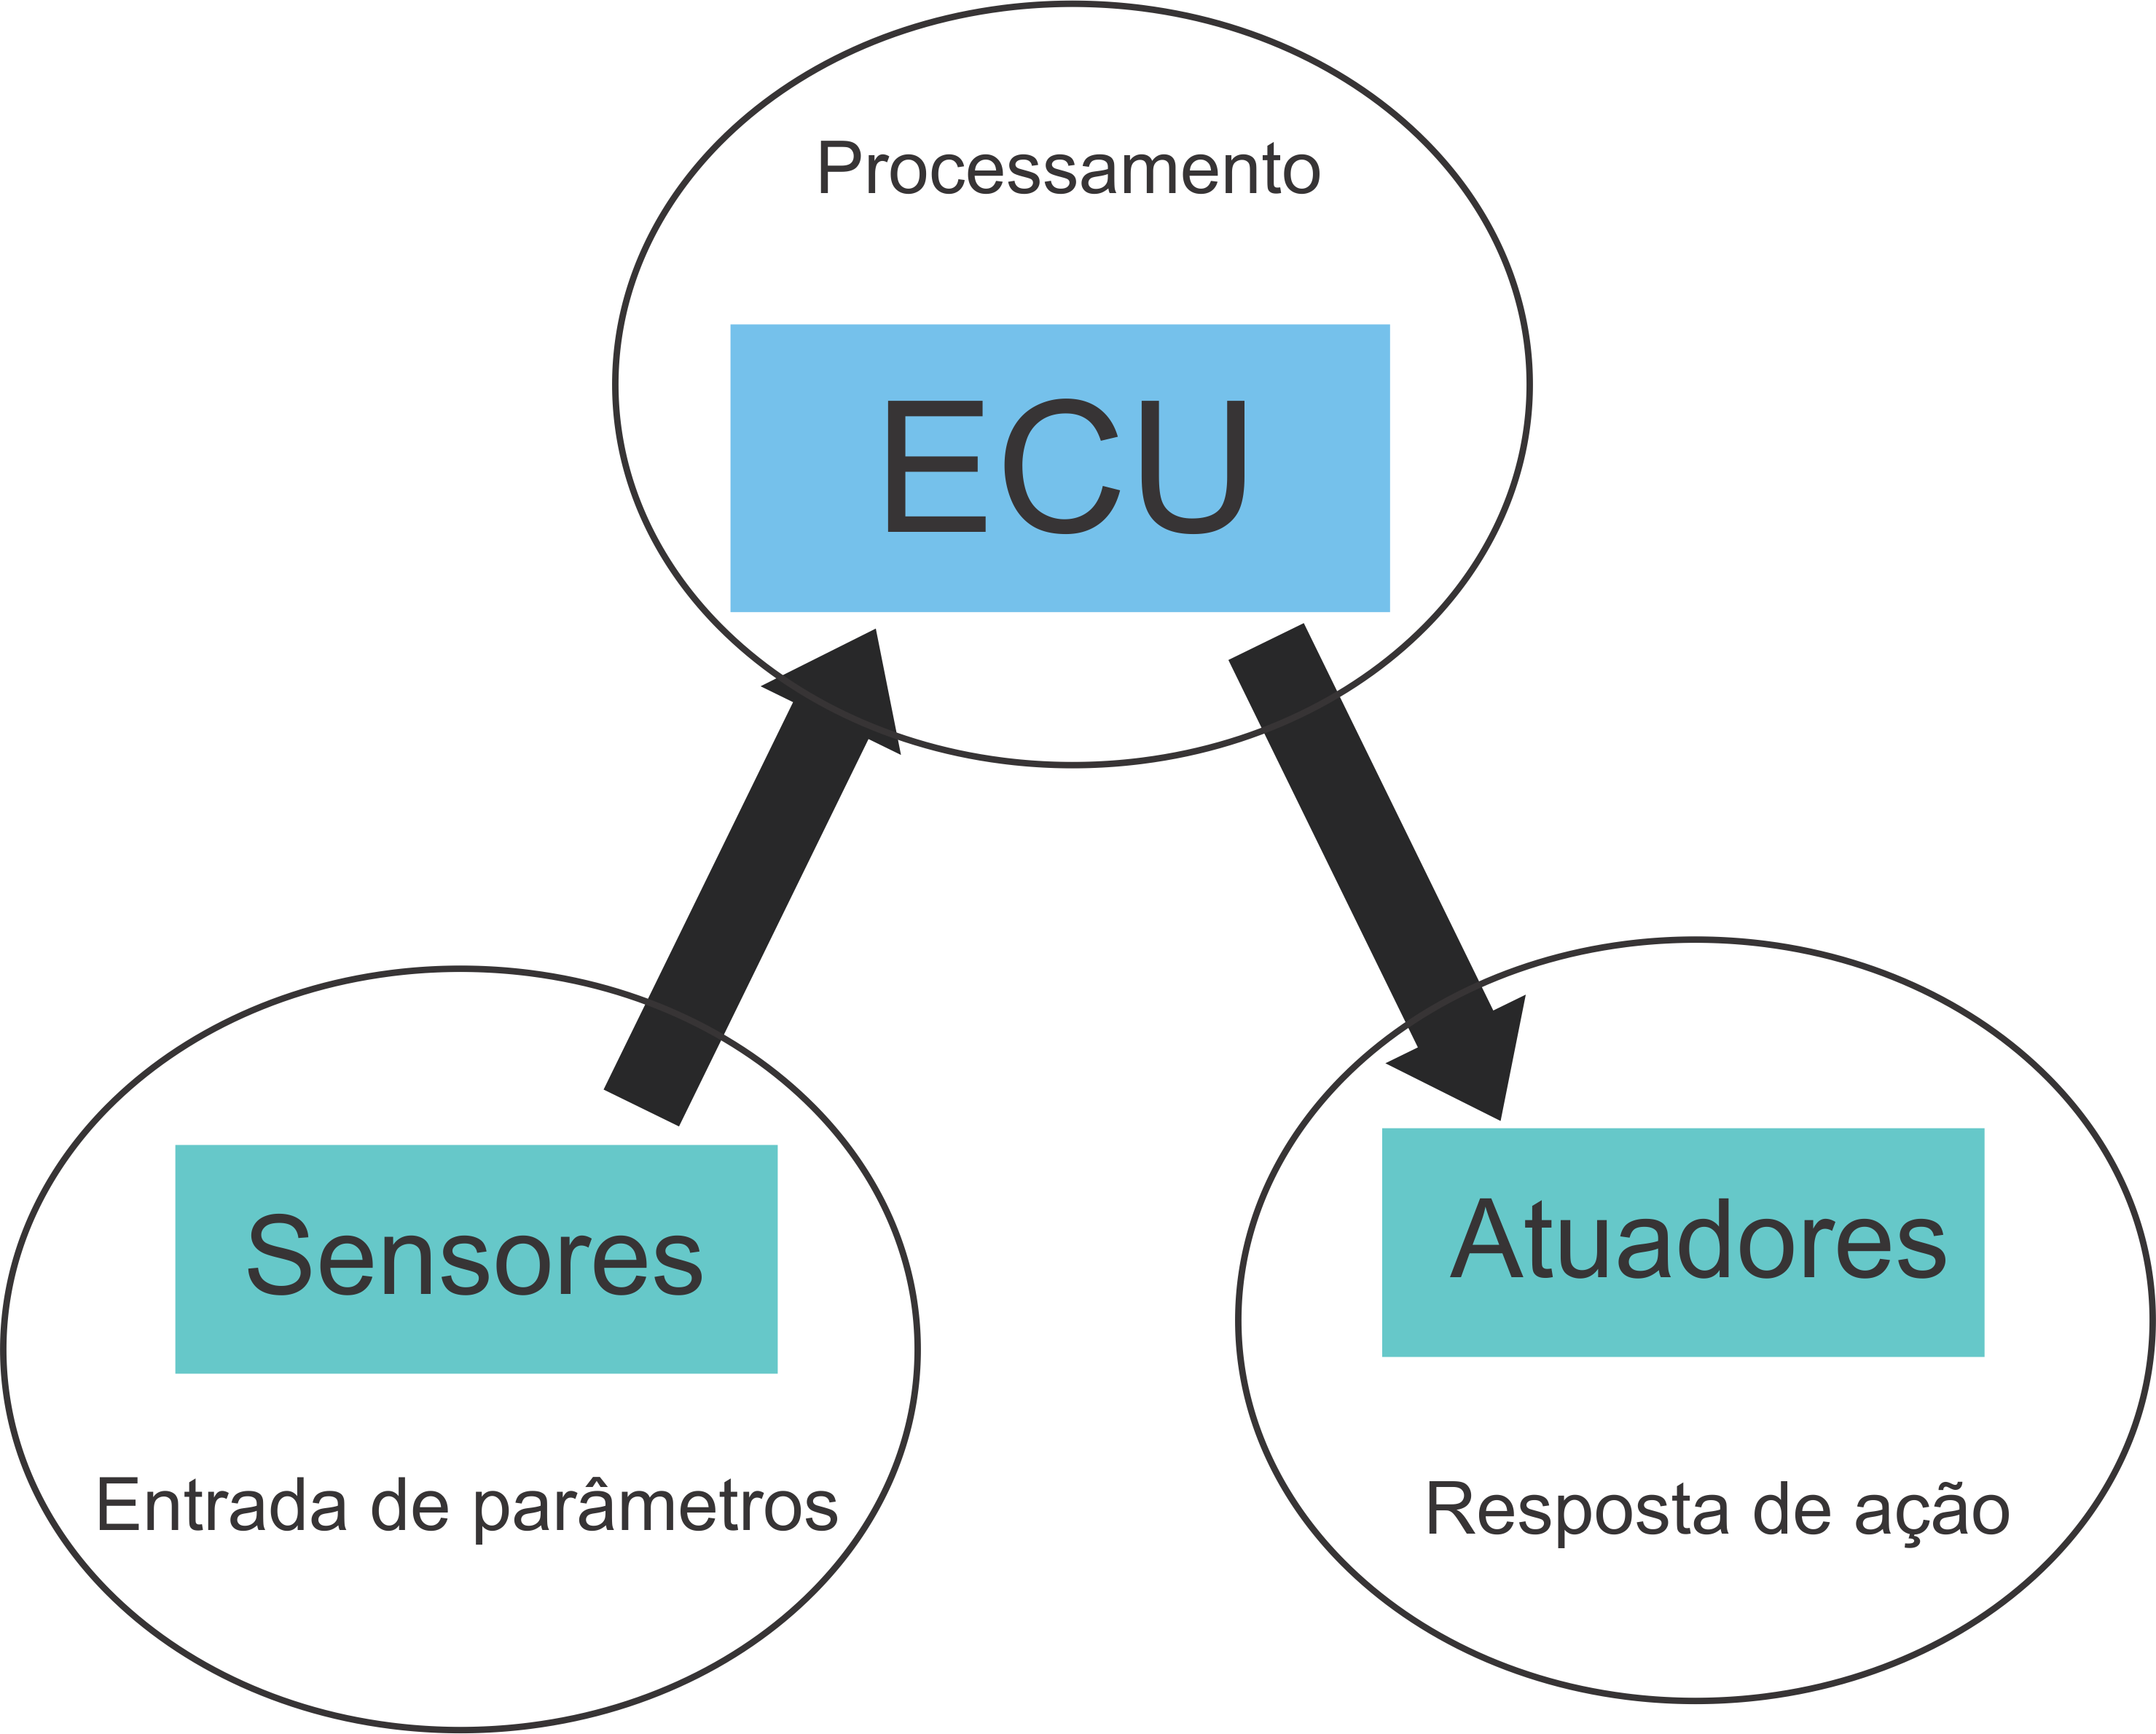
\includegraphics[scale=.34]{imagens/ecuSensorAtuador.png}}\\
\makebox[\width]{Fonte: baseado em \citeonline{navetsimonotlion}} \label{Fig:relacao_ecu_sensor_atuador}
\end{figure}

Segundo Smith, a comunicação da \textit{ECU} com os diversos componentes acontece de forma simplificada. Para esta comunicação ser simples e eficiente, os automóveis utilizam alguns protocolos para tratar da comunicação da rede interna do veículo. Estes protocolos serão explorados na sequência.

\subsection{\textbf{Protocolos automotivos}}
Apesar dos protocolos permitirem a comunicação entre os dispositivos, \citeonline{smith} reforça que caso o veículo tenha sido fabricado antes do ano de 2000, há possibilidade de ele não possuir nenhum protocolo implementado. Para ele, os protocolos presentes nos barramentos são responsáveis por gerenciar a transmissão de pacotes de dados pela rede automotiva. Diversos sensores e dispositivos conectados nesta rede se comunicam com a finalidade de administrar o comportamento do veículo. Segundo o autor, toda a parte da comunicação crítica ocorrem nos barramentos de alta velocidade, enquanto a comunicação não crítica ocorre nos barramentos de média e baixa velocidade. Subentende-se que a comunicação crítica está relacionada a todos os controles que garantem a segurança e integridade dos ocupantes do automóvel. 

\citeonline{navetsimonotlion} afirmam que o papel central das redes está em manter os sistemas embarcados em estado de segurança, uma vez que a maioria das funções críticas estão distribuídas e necessitam da comunicação contínua entre si. Ele ainda aponta que a diversificação das redes utilizadas em todo o automóvel é justificada pela crescente necessidade da largura de banda, desempenho e outros requisitos de confiabilidade.

Cada fabricante decide qual barramento ou protocolo serão utilizados na arquitetura do veículo; entretanto, existe um protocolo comum em todos os veículos: o protocolo \textit{CAN} \cite{smith}. Em 1994, a Sociedade de Engenheiros Automotivos \textit{(Society for Automotive Engineers – SAE)}, citada por \citeonline{navetsimonotlion}, definiu uma classificação para protocolos de comunicação automotiva baseando-se na velocidade de transmissão dos dados e nas funções que seriam distribuídas pela rede (Tabela \ref{tab:tipos_redes_transmissao}). As redes de classe A possuem uma taxa de dados inferior a 10 kbps e são utilizadas para transmissão de dados de controle com tecnologias de baixo custo e estão integradas na categoria \textit{Body}. As redes classe B operam em uma velocidade de 10 a 125 kbps e se dedicam para suportar a troca de dados entre \textit{ECUs}, para reduzir o número de sensores compartilhando informações. Aplicações que precisam de comunicação em tempo real requerem redes de classe C (com velocidade de transmissão de 125 kbps a 1Mbps) ou redes de classe D (operando com velocidades superiores a 1Mbps). As redes classe C integram a comunicação das categorias \textit{Power Train} e \textit{Chassis}. Já as redes de classe D são dedicadas a dados multimídia e aplicações críticas de segurança que requeiram previsibilidade e tolerância de falhas.

\begin{table}[htb!]
\centering
\caption{Tipos de redes e suas respectivas velocidades de transmissão de acordo com a \textit{SAE}.}
\label{tab:tipos_redes_transmissao}
\begin{tabular}{cc}
\hline
Tipos de redes & \multicolumn{1}{c}{Velocidade de transmissão} \\ \hline
Classe A              & até 10 kbps                             \\
Classe B              & de 10 a 125 kbps                          \\
Classe C              & de 125 kbps a 1Mbps                       \\
Classe D              & acima de 1Mbps                            \\ \hline
\end{tabular}
\end{table}

De acordo com \citeonline{navetsimonotlion}, é comum a inclusão dos quatro tipos de redes em barramentos diferentes interligadas por \textit{gateways} na arquitetura eletrônica dos veículos atuais, conforme representado na Figura \ref{Fig:redes_gateway}. Eles ainda complementam que será possível futuramente a inclusão de um barramento dedicado aos sistemas de segurança dos ocupantes. De todos os protocolos existentes e citados pelos autores, serão explorados dois, o protocolo \textit{CAN} e o SAE J1850.

\begin{figure}[!ht]
\centering
\caption{Representação de redes distintas interligadas.} 
{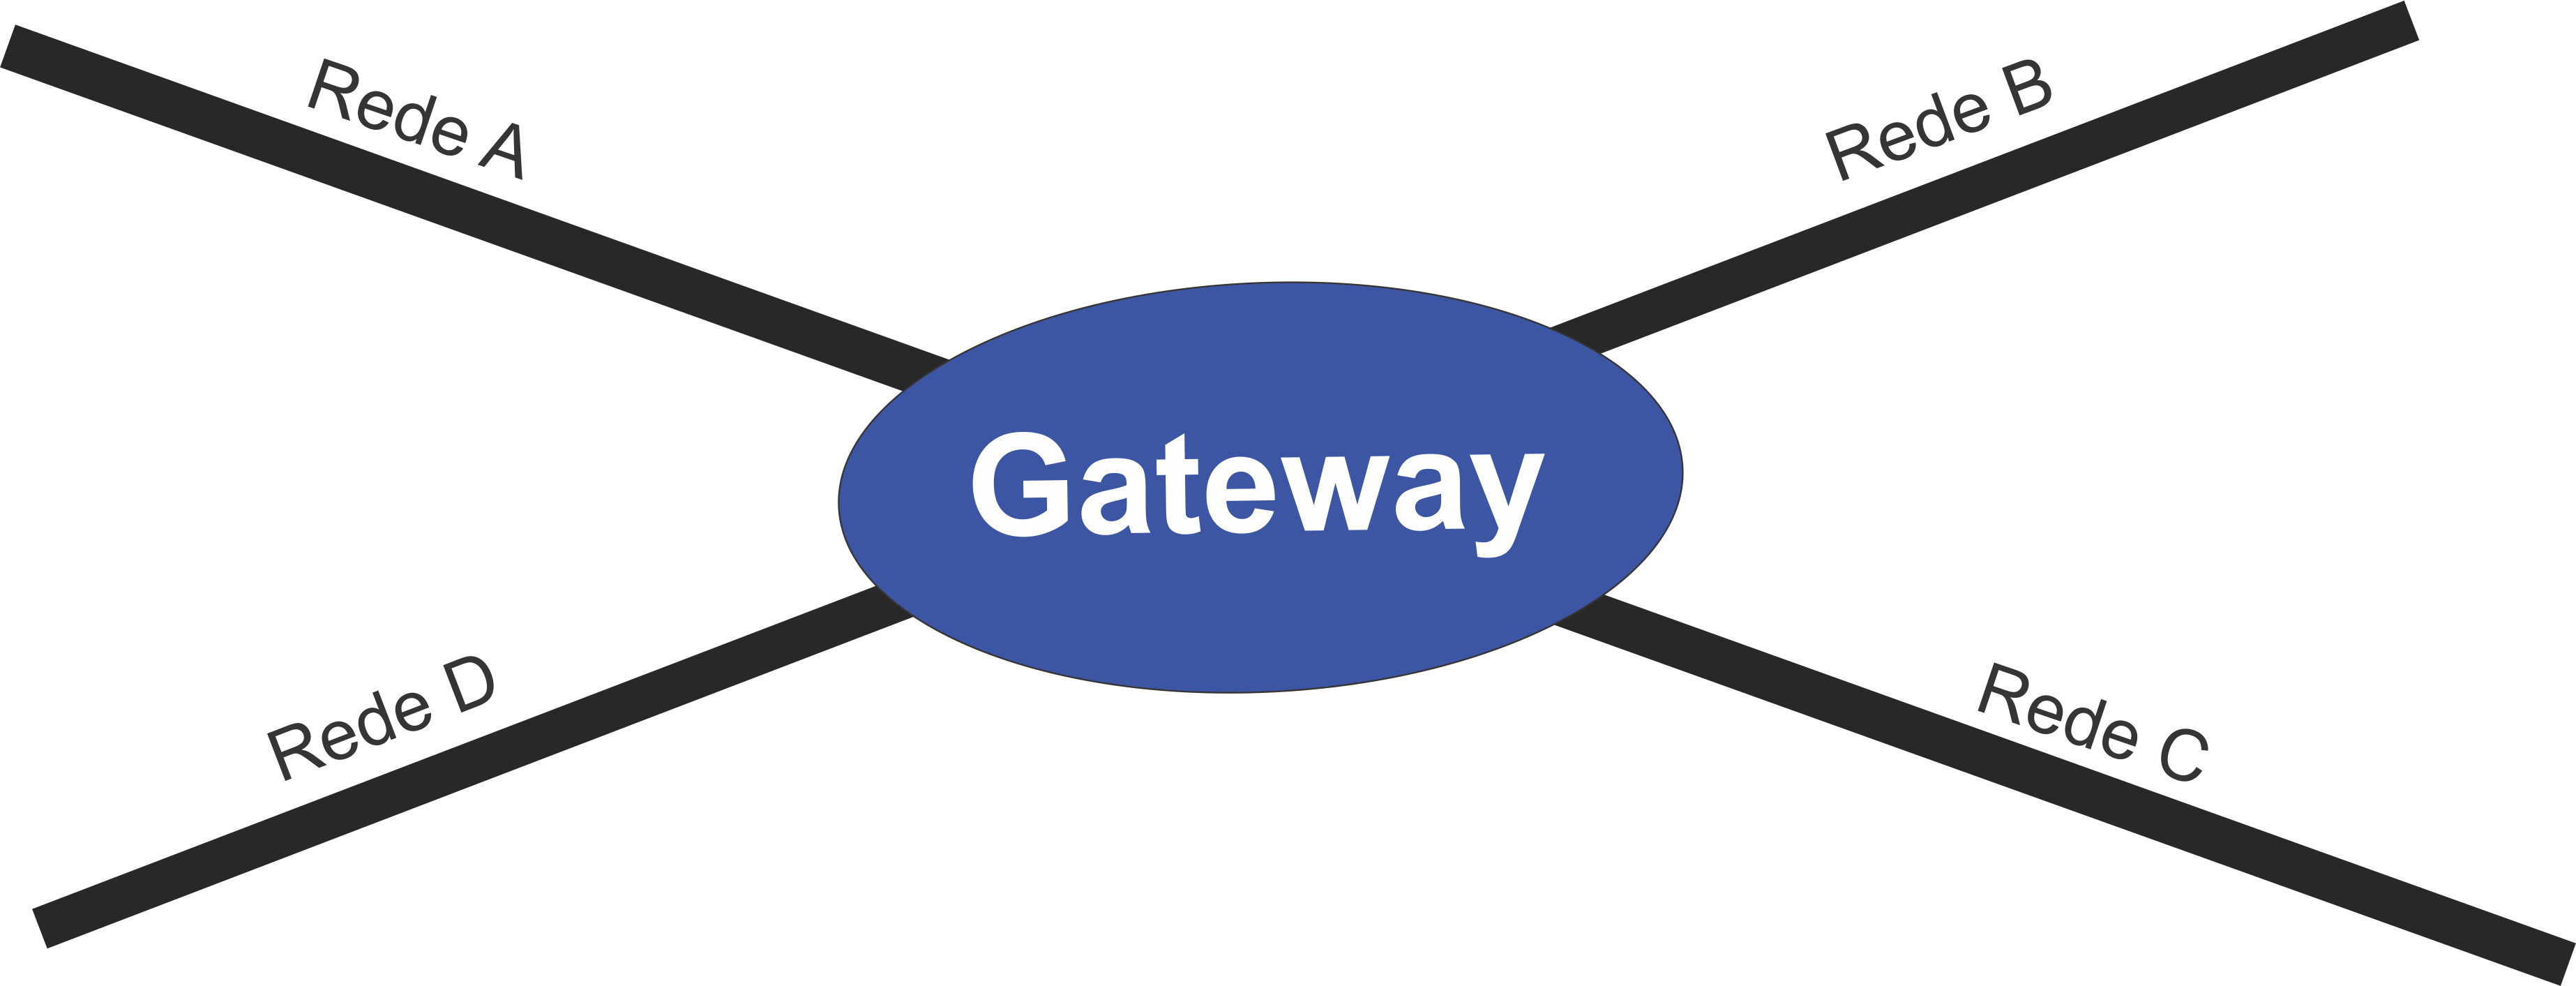
\includegraphics[scale=.35]{imagens/redesGateway.png}}\\
\makebox[\width]{Fonte: baseado em \citeonline{navetsimonotlion}} \label{Fig:redes_gateway}
\end{figure}

\subsubsection{\underline{\textbf{Protocolo \textit{CAN} \textit{(Controller Area Network)}}}}
Por volta de 1980, foi desenvolvido pela Bosch o protocolo conhecido como \textit{CAN} \textit{(Controller Area Network)}, ou simplesmente protocolo de controle de área de rede. Este protocolo foi integrado pela primeira vez em carros de produção da Mercedes na década de 90 \cite{navetsimonotlion}. \citeonline{smith} afirma que o \textit{CAN} é um protocolo simples utilizado na indústria automobilística. Este protocolo permite a comunicação de \textit{ECUs} e sistemas embarcados que estão presentes nos veículos modernos. \citeonline{navetsimonotlion} ainda complementam que as redes que utilizam esse protocolo tornaram-se as mais utilizadas nos sistemas automotivos. Por possuírem baixo custo, serem robustas e terem atrasos baixos de comunicação, o protocolo \textit{CAN} é um padrão utilizado na Europa para transmissão de dados de aplicações automotivas.

Atualmente, para controlar os sistemas da categoria \textit{Power Train} utiliza-se a \textit{CAN} como uma rede \textit{SAE} de classe C, operando de 250 a 500 kbps. Entretanto, ela também pode operar nos sistemas de categoria \textit{Body}, com uma taxa de 125 kbps. Segundo os estudos de \citeonline{smith}, o protocolo \textit{CAN} possui dois tipos de pacotes que são chamados de \textit{standard} (padrão) e \textit{extended} (extendido).

Os pacotes \textit{standard} possuem quatro elementos, que são o ID de arbitragem, extensão de ID, código do tamanho dos dados e os própios dados. Quando um dispositivo tenta se comunicar é enviado ID de arbitragem, que é uma mensagem de broadcast que identifica o ID deste dispositivo. Quando dois pacotes são transmitidos ao mesmo tempo no barramento, aquele com ID de arbitragem menor vence. \citeonline{navetsimonotlion} apontam esta técnica como sendo um método utilizado por este protocolo para evitar colisões ao acessar o barramento. Voltando aos estudos de \citeonline{smith}, ele afirma que o bit que define a extensão de ID tem o valor 0 para pacotes \textit{standard}. O código do tamanho dos dados define o tamanho dos dados, que pode variar de 0 a 8 bytes. O tamanho máximo dos dados transportados por este pacote pode ter no máximo 8 bytes.

Já os pacotes \textit{extended}, segundo o autor, são semelhantes ao \textit{standard}, com exceção de possuir espaço maior para armazenar IDs mais longos. Estes pacotes foram desenvolvidos para caberem dentro do formato \textit{standard} para manter a compatibilidade com as versões anteriores. Desta forma, caso algum sensor tenha suporte somente para pacotes \textit{standard}, ele não será invalidado caso sejam transmitidos pacotes \textit{extended} na mesma rede. Dentre outras particularidades deste pacote, \citeonline{smith} ainda reforça que existem outros protocolos adicionais específicos de alguns fabricantes (protocolo ISO-TP, \textit{CANopen}, GMLAN) que seguem o padrão \textit{CAN}, da mesma forma que o pacote \textit{CAN} \textit{extended} (Figura \ref{Fig:implementacoes_can}).

\begin{figure}[!ht]
\centering
\caption{Representação de outros protocolos implementados no padrão \textit{CAN}.} 
{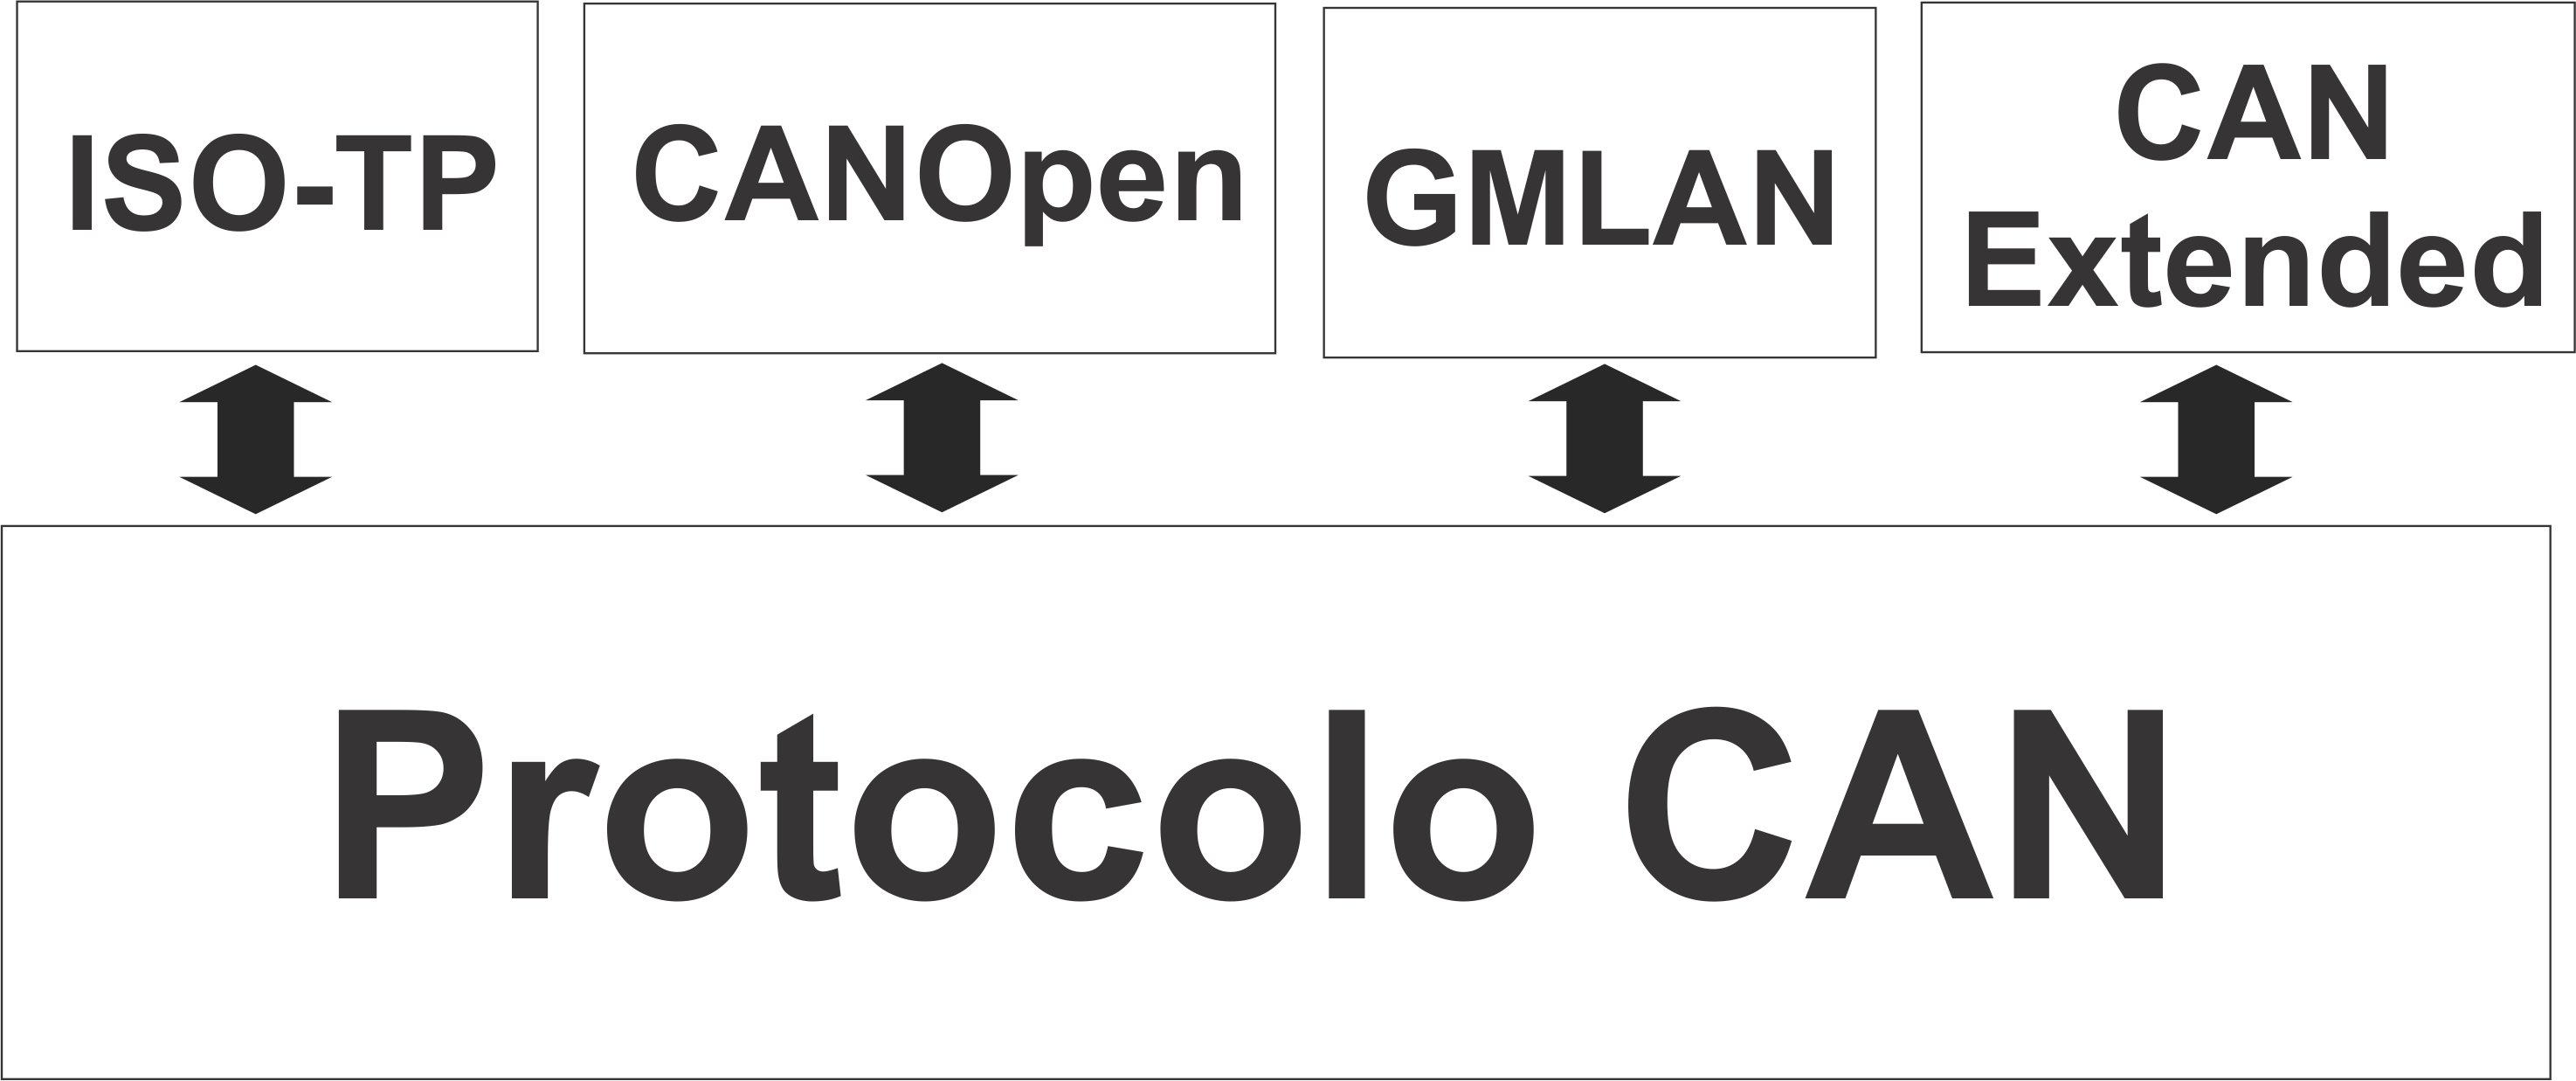
\includegraphics[scale=.25]{imagens/protocoloCanEVariacoes.png}}\\
\makebox[\width]{Fonte: baseado em \citeonline{smith}} \label{Fig:implementacoes_can}
\end{figure}

Segundo \citeonline{navetsimonotlion}, o protocolo \textit{CAN} define apenas a camada física e a camada de link dos dados. Para tratar a padronização de inicialização, implementar a segmentação de dados ou enviar mensagens periódicas, foram propostos diversos protocolos de nível superior.

\subsubsection{\underline{\textbf{Protocolo SAE J1850}}}
O protocolo SAE J1850 foi implementado originalmente por volta de 1994, segundo \citeonline{smith}, e ainda pode ser encontrado nos veículos atuais. Comparado com o protocolo \textit{CAN}, este é mais lento, entretanto, seu custo de implantação é mais barato. \citeonline{navetsimonotlion} menciona que são definidas duas variações para este protocolo. \citeonline{smith} as define como modulação de largura de pulso \textit{(pulse width modulation – PWM)} e largura de pulso variável \textit{(variable pulse width – VPW)}, conforme representado pela Figura \ref{Fig:implementacoes_saej1850}. O \textit{PWM} trabalha com uma velocidade de 41.6 Kbps, enquanto o \textit{VPW} trabalha com 10.4 Kbps.

\begin{figure}[!ht]
\centering
\caption{Variações do protocolo SAE J1850.} 
{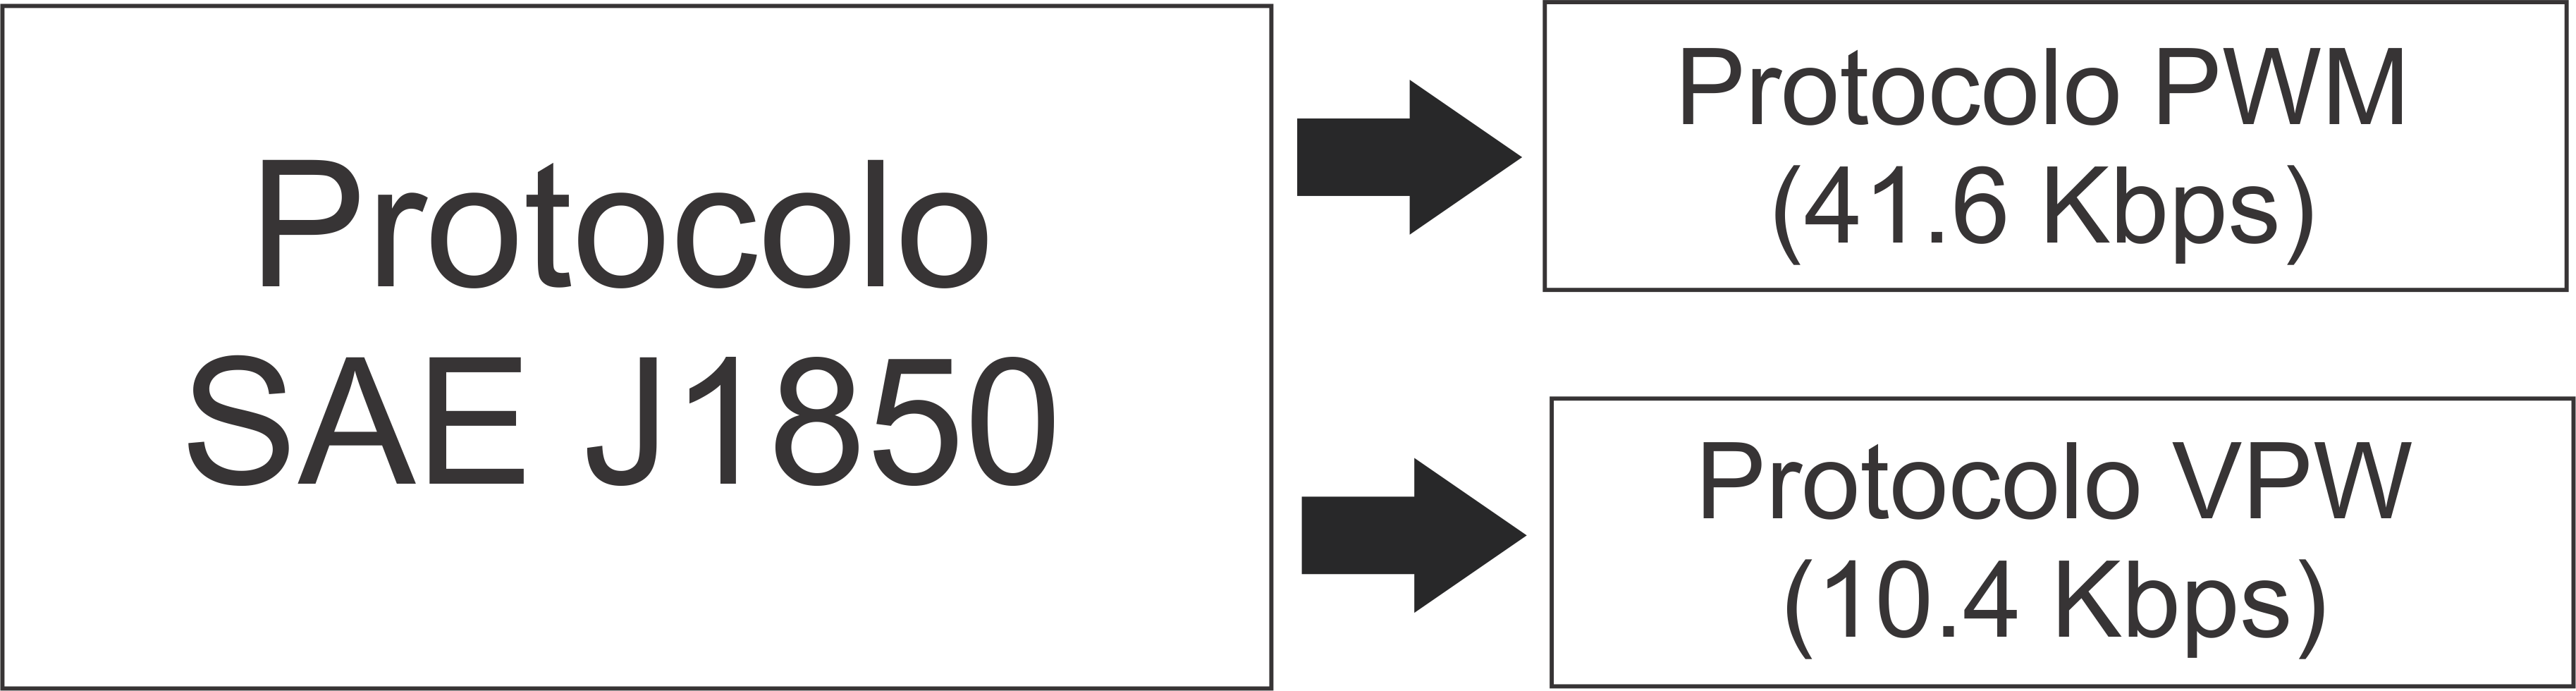
\includegraphics[scale=.25]{imagens/protocoloSaeJ1850.png}}\\
\makebox[\width]{Fonte: baseado em \citeonline{smith, navetsimonotlion}} \label{Fig:implementacoes_saej1850}
\end{figure}

\citeonline{navetsimonotlion} afirmam que para tratar dos controles dos sistemas da categoria \textit{Body} ou de diagnósticos, os Estados Unidos adotaram este protocolo SAE J1850 de classe B pois as comunicações não possuíam requisitos de transmissão em tempo real.

Analisando os protocolos apresentados, observa-se que para determinada aplicação é utilizado um protocolo específico.  E cada protocolo tem uma classificação quanto à sua velocidade de transmissão pelo \textit{SAE}. Existem outros protocolos que estão presentes na rede automotiva, como o \textit{Keyword Protocol} e ISO 9141-2, explorados por \citeonline{smith}, os protocolos IDB-1394, \textit{VAN (Vehicle Area Network)} e \textit{TTCAN}, explorados por \citeonline{navetsimonotlion}, ou ainda os protocolos \textit{LIN (Local Interconnect Protocol)}, \textit{MOST (Media Oriented Systems Transport)} e o \textit{FlexRay}, todos explorados na literatura de ambos.

Observando-se o comportamento da rede automotiva, nota-se a presença de vários protocolos responsáveis pela comunicação de diversos dispositivos que são destinados a realizar uma determinada função específica no veículo. Entretanto, também existe a necessidade de monitorar essa rede para realizar eventuais diagnósticos neste sistema, e o nome dado para esta função se chama diagnóstico de bordo \textit{(OnBoard Diagnostics – OBD)} \cite{navetsimonotlion}.

\subsection{\textbf{Conector \textit{OBD-II (OnBoard Diagnostics)}}}\label{subsecaoobd}
Também conhecido como conector de diagnóstico de conexão \textit{(Diagnostic Link Connector – DLC)}, o conector \textit{OBD-II} está integrado em grande parte dos veículos, e permite a comunicação com a rede interna automotiva conforme exemplificado por \citeonline{smith}. De acordo com \citeonline{navetsimonotlion}, a introdução de sistemas informáticos capazes de memorizar grandes quantidades de informação de um automóvel possibilitou o diagnóstico de bordo, que se refere ao autodiagnóstico e a facilidade de emissão de relatórios. Para \citeonline{smith}, o conector \textit{OBD-II} é utilizado principalmente pela mecânica para analisar e solucionar eventuais problemas com o automóvel. A Figura \ref{Fig:obd2} mostra a localização do conector \textit{OBD-II} em um automóvel.

\begin{figure}[!ht]
\centering
\caption{Foto do conector \textit{OBD-II}.} 
{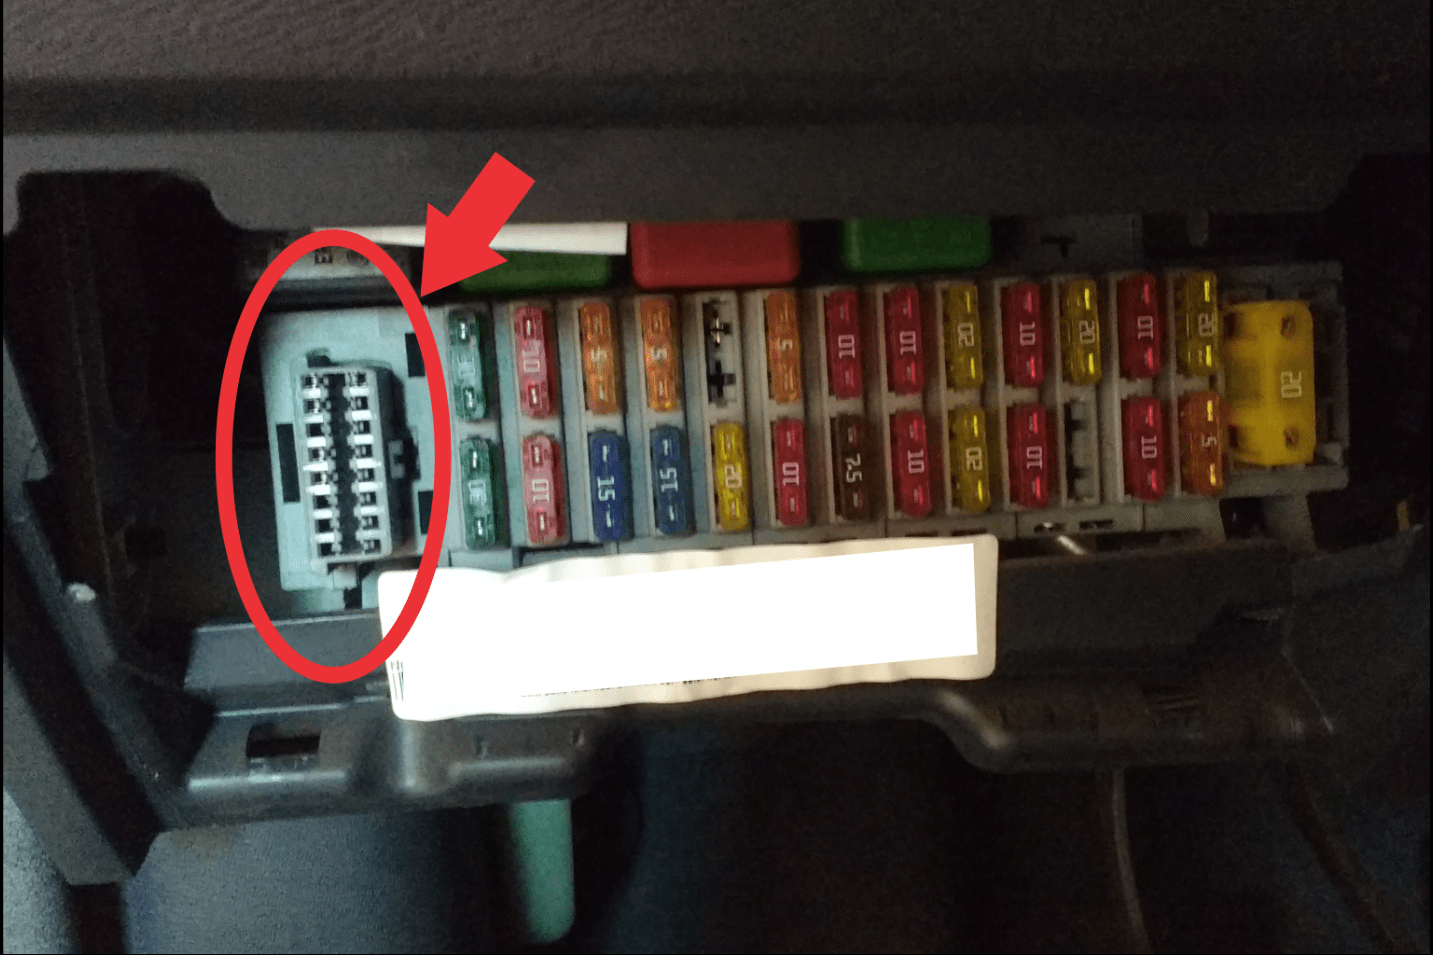
\includegraphics[scale=.19]{imagens/obdII.png}}\\
\makebox[\width]{Fonte: foto tirada pelo autor} \label{Fig:obd2}
\end{figure}

Ao apresenta uma falha, o sistema guarda informações relacionadas a ela e aciona uma luz de aviso do motor no painel do motorista, conhecida como luz indicadora de mau funcionamento (\textit{malfunction indicator lamp – MIL}, Figura \ref{Fig:luz_mil}). Embora o diagnóstico tenha se limitado a essa luz indicadora, conforme \citeonline{navetsimonotlion} apresentam, a comunicação dos sistemas \textit{OBD} recentes são padronizados, como por exemplo a padronização de dados monitorados, codificação padronizada e relatórios de uma lista de falhas específicas, conhecidas como códigos de diagnósticos de problemas \textit{(Diagnostic Trouble Codes – DTC)}. De acordo com \citeonline{smith}, as verificações de rotina são tratadas pela \textit{ECU} primária do veículo, o qual ele se refere de módulo de controle do \textit{powertrain} \textit{(PCM)}. Para controlar a emissão de gases de escape ao longo da vida útil de um veículo, segundo \citeonline{navetsimonotlion}, foi necessário uma padronização na especificação \textit{OBD-II}, que passou a ser obrigatória para todos os carros comercializados nos Estados Unidos a partir de 1996. Este padrão definia com precisão diversos aspectos relacionados ao diagnóstico, avaliação e monitoramento do veículo.

\begin{figure}[!ht]
\centering
\caption{Foto da luz \textit{MIL} do painel.} 
{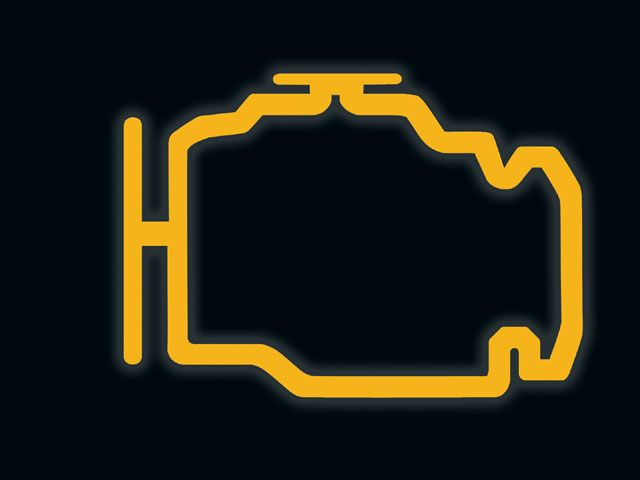
\includegraphics[scale=.15]{imagens/luzMil.jpg}}\\
\makebox[\width]{Fonte: imagem extraída do site https://goo.gl/CiSaec} \label{Fig:luz_mil}
\end{figure}

Voltando à parte de diagnósticos, com base nos estudos de \citeonline{smith}, todos os códigos de falha, como os \textit{DTCs} são armazenados no \textit{PCM}. Ele ainda complementa dizendo que os \textit{DTCs} são armazenados em locais diferentes. Enquanto os \textit{DTCs} baseados em memória ficam armazenadas na memória RAM e apagados quando a energia da bateria acaba, os \textit{DTCs} mais sérios que estão relacionados com falhas permanentes ficam armazenados em locais onde a persistência de dados é maior e consequentemente sobreviverão à uma queda de energia.

A Figura \ref{Fig:rede_veicular} representa de maneira simplificada como ocorre a comunicação entre os dispositivos na rede interna automotiva.

\begin{figure}[!ht]
\centering
\caption{Diagrama representando a arquitetura da rede veicular.} 
{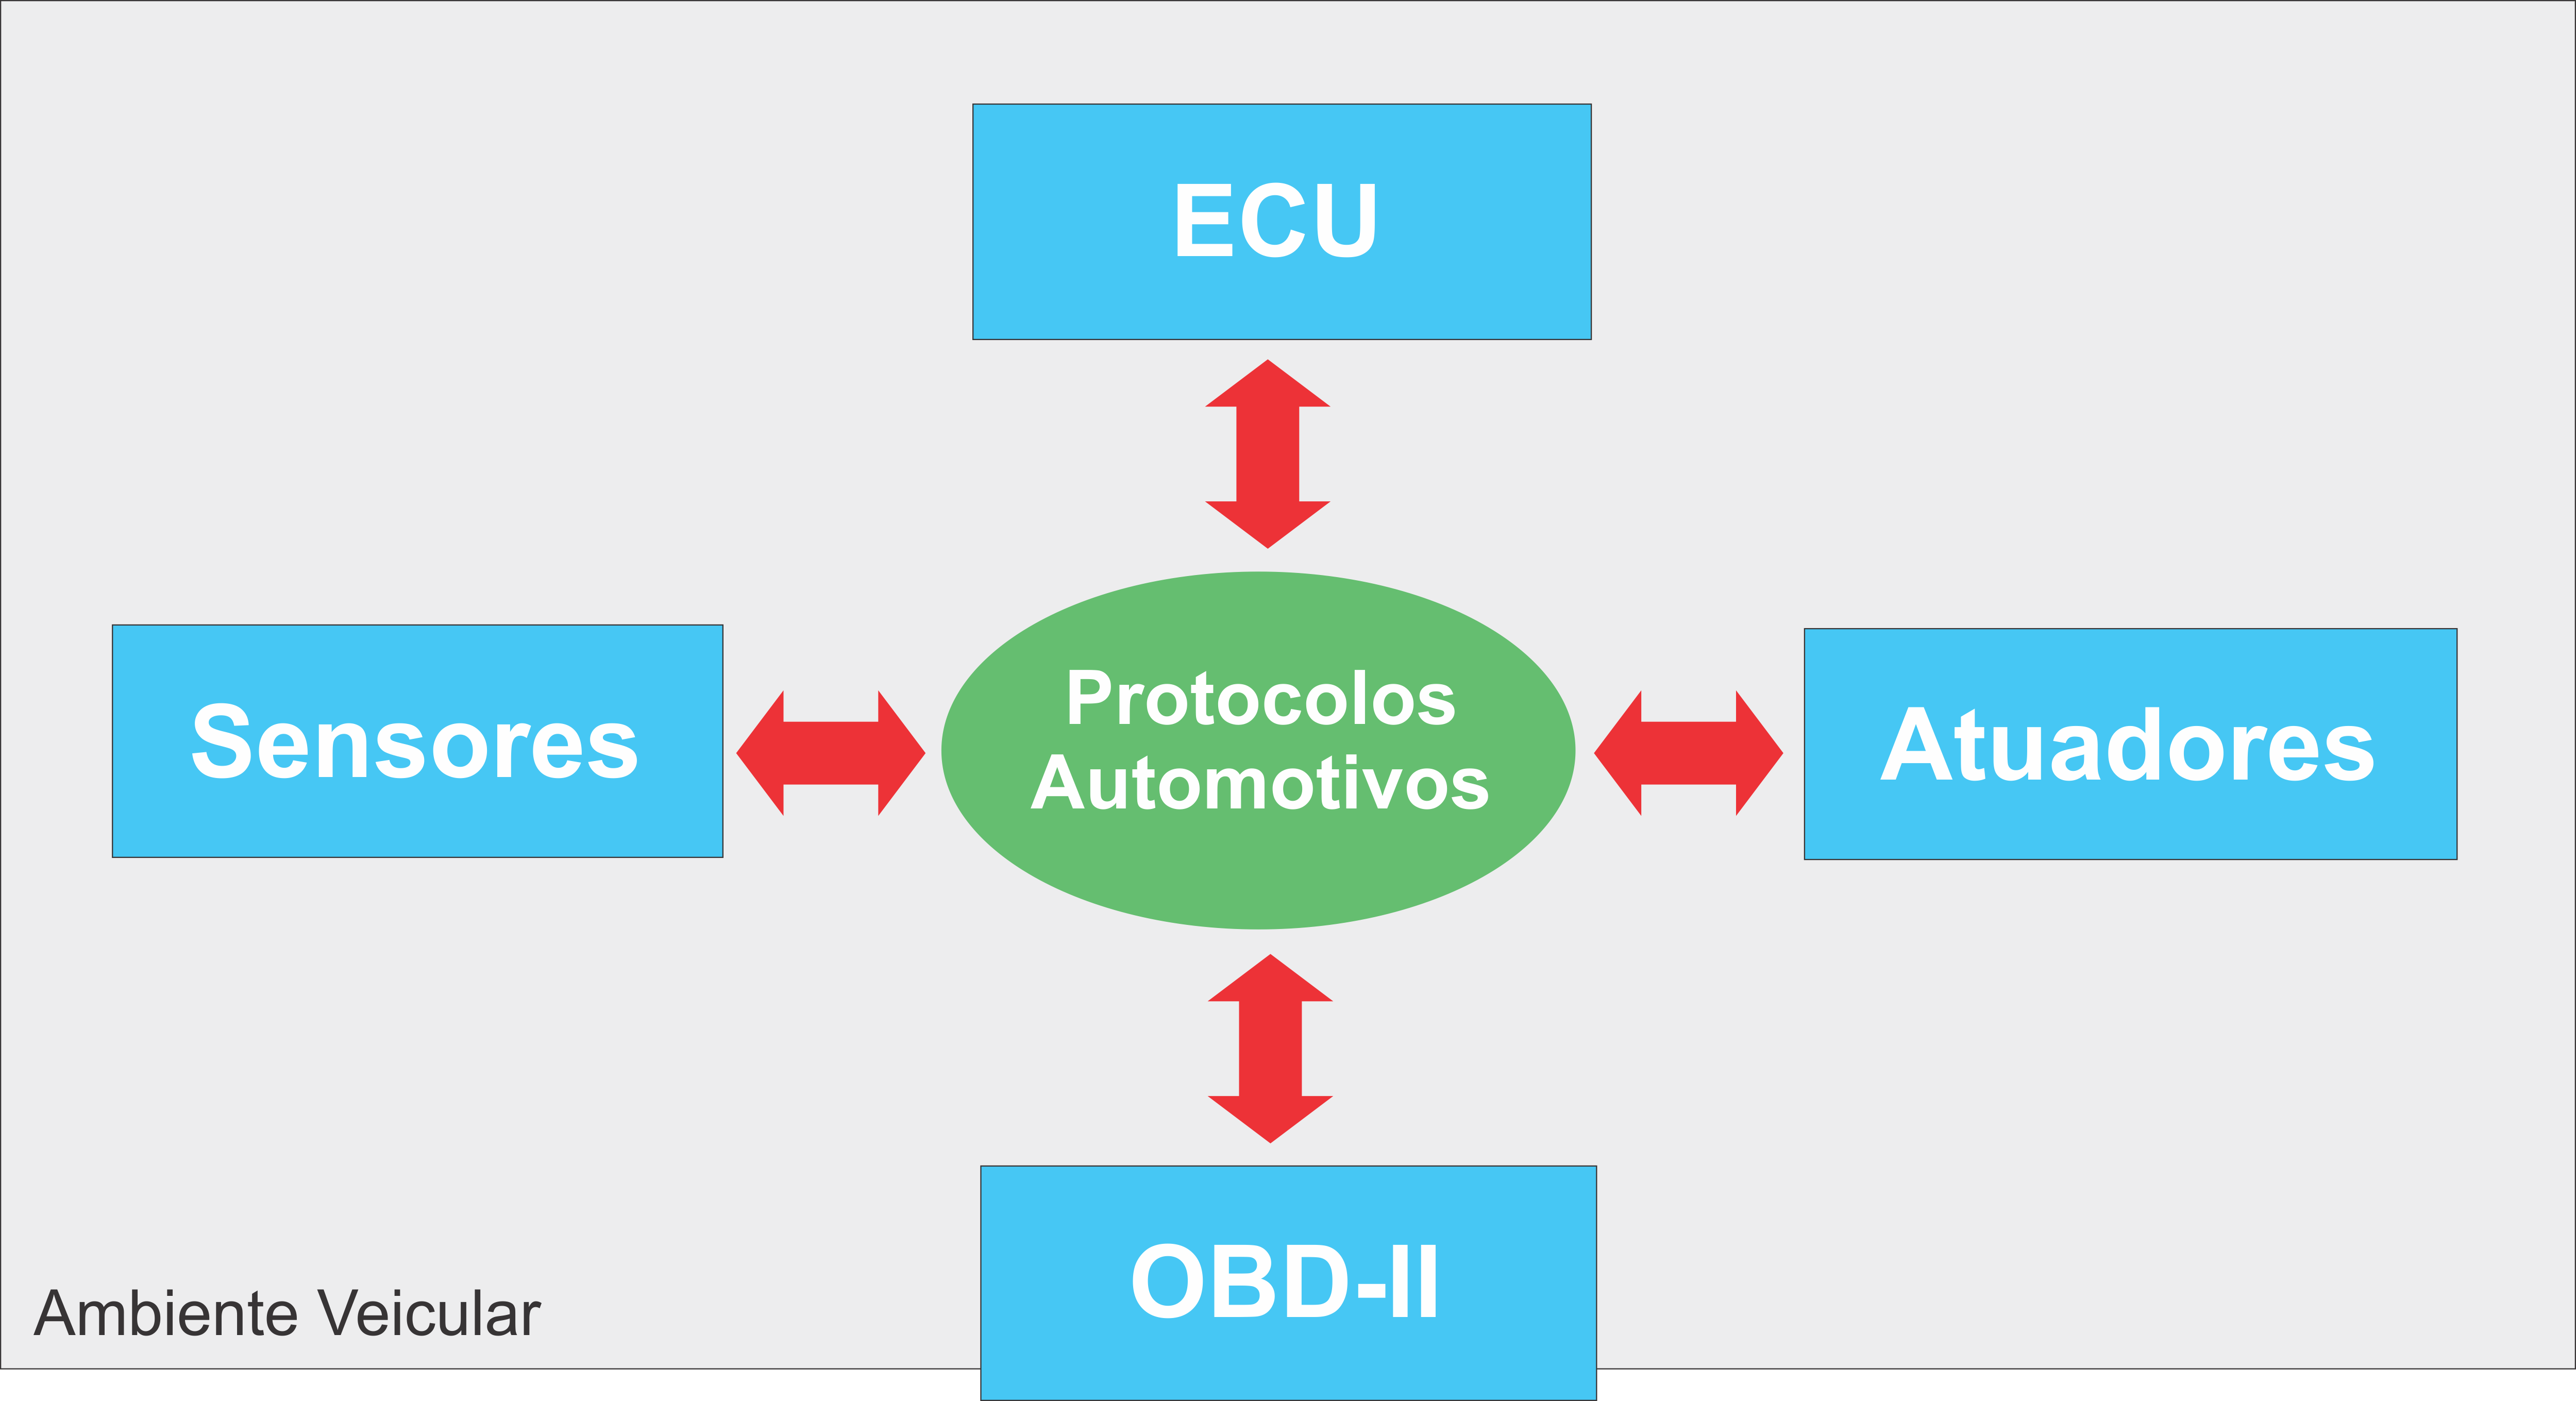
\includegraphics[scale=.32]{imagens/arquiteturaRedeVeicular.png}}\\
\makebox[\width]{Fonte: baseado em \citeonline{navetsimonotlion} e \citeonline{smith}} \label{Fig:rede_veicular}
\end{figure}

\section{ELM327}
A lei atualmente obriga, segundo a \citeonline{elmeletronics}, que todos os automóveis produzidos forneçam uma interface para a conexão de dispositivos de teste e diagnóstico. Esta interface apresentada na subseção \ref{subsecaoobd} como \textit{OBD-II}, segue as mesmas especificações dos protocolos da rede interna automotiva, o que permite a interação com ela somente se utilizar os mesmos padrões que foram estabelecidos por esta rede. Entretanto, a \citeonline{elmeletronics} ressalta que tais padrões não são compatíveis com computadores ou outros dispositivos inteligíveis, como um smartphone, por exemplo. Para solucionar este problema e permitir a compatibilidade, o ELM327 foi desenvolvido para servir de intermediário entre a porta \textit{OBD-II} - presente nos automóveis - com a interface serial padrão (RS232) presente nos computadores. A \citeonline{elmeletronics} ainda afirma que este dispositivo é capaz de identificar e interpretar nove protocolos automotivos mais o padrão J1939 utilizado por ônibus e caminhões. Desta maneira, com o ELM327 é possível utilizar um computador para se comunicar com a rede interna de um automóvel.

O ELM327 se conecta ao computador por meio da interface serial, que segundo a \citeonline{elmeletronics}, esta interface pode ser virtualizada com adaptadores USB, ou por meio de dispositivos com suporte \textit{bluetooth}. O fabricante reforça que o meio que o dispositivo usa para se conectar ao computador não tem muita relevância, pois para se comunicar com o veículo através da rede, basta apenas uma aplicação que faça o envio ou recebimento dos dados. Entretanto, para garantir a comunicação, alguns ajustes devem ser configurados, como a configuração da porta e a taxa de dados correta, conforme abordados no manual. A Figura \ref{Fig:elm327} mostra como é um dispositivo ELM327 \textit{Bluetooth}, e a Figura \ref{Fig:rede_veicular_elm327} expressa como este dispositivo se integra com o automóvel.

\begin{figure}[!ht]
\centering
\caption{Foto do ELM327 \textit{Bluetooth}.} 
{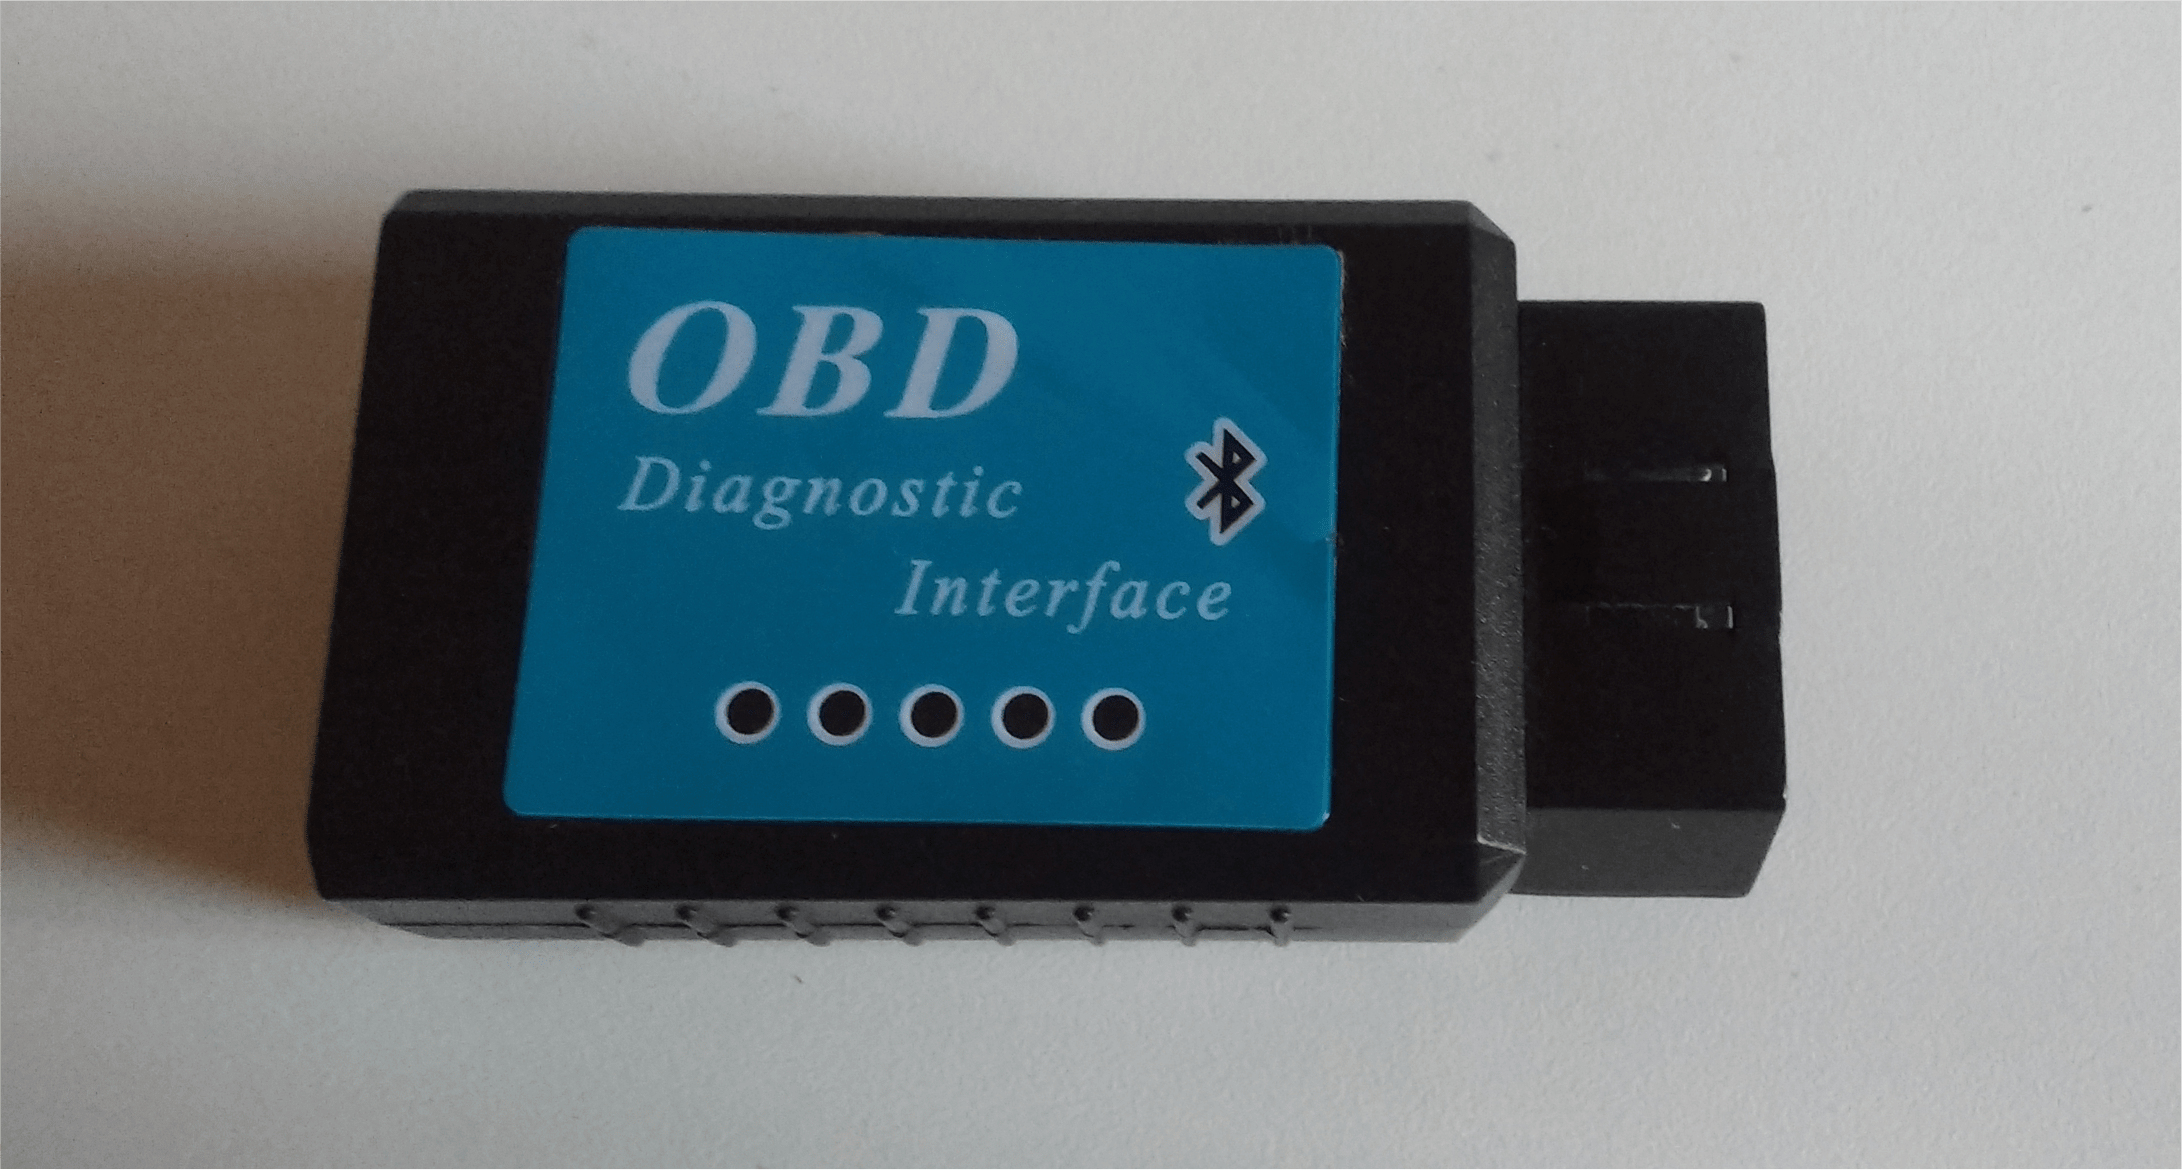
\includegraphics[scale=.16]{imagens/elm327-min.png}}\\
\makebox[\width]{Fonte: foto tirada pelo autor} \label{Fig:elm327}
\end{figure}

\begin{figure}[!ht]
\centering
\caption{Diagrama representando a interação do ELM327 com a rede automotiva.} 
{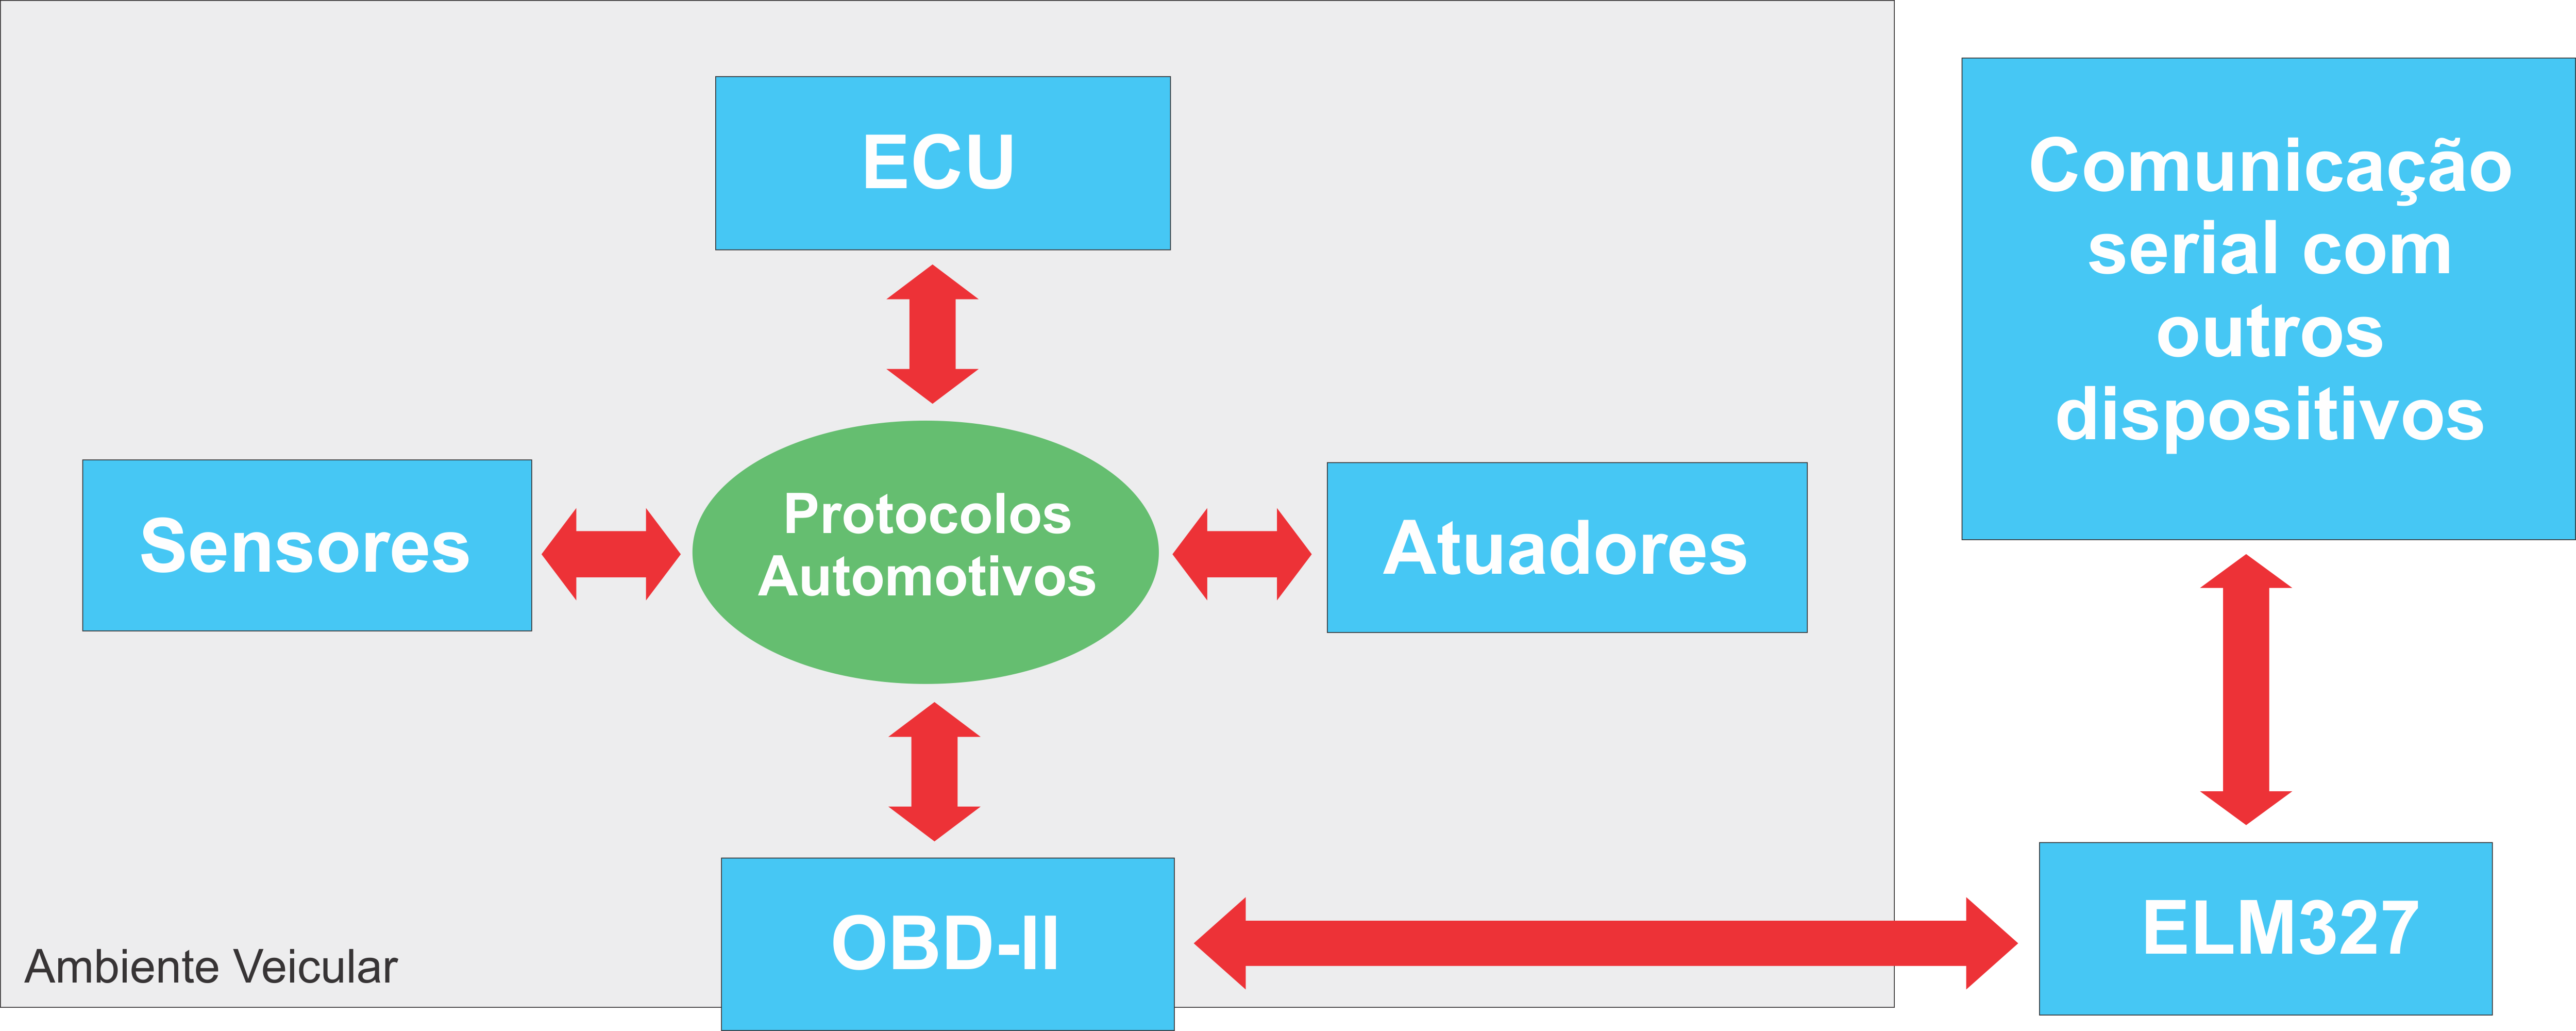
\includegraphics[scale=.35]{imagens/arquiteturaRedeVeicularELM327.png}}\\
\makebox[\width]{Fonte: baseado em \citeonline{elmeletronics}} \label{Fig:rede_veicular_elm327}
\end{figure}

Existem dois tipos de comandos que podem ser enviados. Os comandos que se destinam ao próprio dispositivo, e os comandos destinados ao veículo. Segundo a \citeonline{elmeletronics}, os comandos destinados ao dispositivo começam com os caracteres ‘AT’, enquanto os destinados à rede veicular contêm dígitos hexadecimais. Ele ainda ressalta que o ELM327 apenas converte os protocolos, não realizando nenhum tipo de validação dos dados transmitidos. Entretanto, este dispositivo garante a entrega dos dados nas extremidades, ou seja, garante que os dados sejam transmitidos tanto para o computador quanto para o veículo.

\subsection{\textbf{Comandos AT}}
Como visto anteriormente, os comandos ‘AT’ são destinados ao próprio dispositivo ELM327. Existem vários parâmetros dentro dele que podem ser ajustados para modificar seu comportamento, segundo o fabricante. Esses comandos são semelhantes aos utilizados pelos modems para a configuração interna \cite{elmeletronics}.

\subsection{\textbf{Comandos \textit{OBD}}}
Quando um comando é enviado sem as iniciais ‘AT’, é entendido como comando \textit{OBD} para o veículo. Desta forma, o dispositivo apenas verifica se o comando enviado é um algarismo hexadecimal ou uma sequencia aleatória de caracteres, e logo após transmite o dado ao veículo. Para a \citeonline{elmeletronics}, estes dados são empacotados e enviados ao automóvel. Os comandos enviados ao veículo necessitam geralmente de mais quatro bytes adicionais: três bytes de cabeçalho e um byte de verificação de erro, que devem ser incluídos junto aos dados que serão enviados. Contudo, o ELM327 adiciona estes bytes extras ao comando, abstraindo esta necessidade do usuário.

O comprimento dos comandos \textit{OBD} pode variar de um a sete bytes, sendo este último o limite máximo aceito pelo dispositivo. Ao empacotar e enviar o comando pela interface \textit{OBD}, o dispositivo fica monitorando o barramento veicular para obter a resposta ao comando. Obtida a resposta, ela será encaminhada para a porta serial ao usuário.

\subsubsection{\underline{\textbf{Comunicação com o veículo - padrões de solicitação}}}
De acordo com a \citeonline{elmeletronics}, o formato das solicitações que são enviadas ao veículo devem seguir um padrão definido. O primeiro byte enviado é denominado ‘modo’ \textit{(mode)}. Este byte informa que tipo de dados está sendo solicitado. O segundo byte é conhecido como ID de parâmetro, ou simplesmente número PID \textit{(parameter identification)}. Este especifica a informação real que é necessária, como acessar uma informação de um determinado dispositivo do automóvel, por exemplo. Os modos e PIDs são descritos em detalhes pelos padrões SAE J1979 ou ISO 15031-5, além de poderem ser definidos também pelos fabricantes dos automóveis. Entretanto, como menciona a \citeonline{elmeletronics}, é comum um veículo não suportar todos os ‘modos’ e PIDs descritos pelo padrão. As mensagens de resposta, que geralmente são enviadas pela \textit{ECU}, são retornadas em conjunto de números hexadecimais, havendo a necessidade de realizar algumas conversões para ter acesso aos valores que foram retornados. Uma segunda conversão é necessária de acordo com o PID que foi solicitado (a conversão do valor varia de acordo com o PID).

\section{\textit{RASPBERRY PI}}
Segundo \citeonline{oliveira}, o \textit{Raspberry Pi} veio ao mercado com a proposta de ser um equipamento barato e dar suporte ao processo educacional das crianças. Segundo uma entrevista de Torvalds\nocite{torvalds} ao site \textit{BBC News} em 2012, o projeto \textit{Raspberry Pi} é algo importante, pois por ser de baixo custo, permite a exploração da informática sem a preocupação com possíveis danos ao hardware.

\citeonline{richardsonwallace} afirmam que é possível realizar diversas atividades com o \textit{Raspberry Pi}, como utilizá-lo para computação de maneira geral, aprender programação ou ainda integrar o minicomputador a projetos eletrônicos. Segundo os autores, um dos fatores que o diferenciam de um computador convencional além do seu tamanho e preço, é sua facilidade de integração com projetos eletrônicos. Apesar de parecer semelhante aos microcontroladores, as plataformas \textit{System on a Chip (SoC)} possuem mais características em comum com um computador do que com um microcontrolador qualquer. A Figura \ref{Fig:raspberry_pi} mostra a aparência física do \textit{Raspberry Pi}.

\begin{figure}[!ht]
\centering
\caption{Foto do \textit{Raspberry Pi} 3.} 
{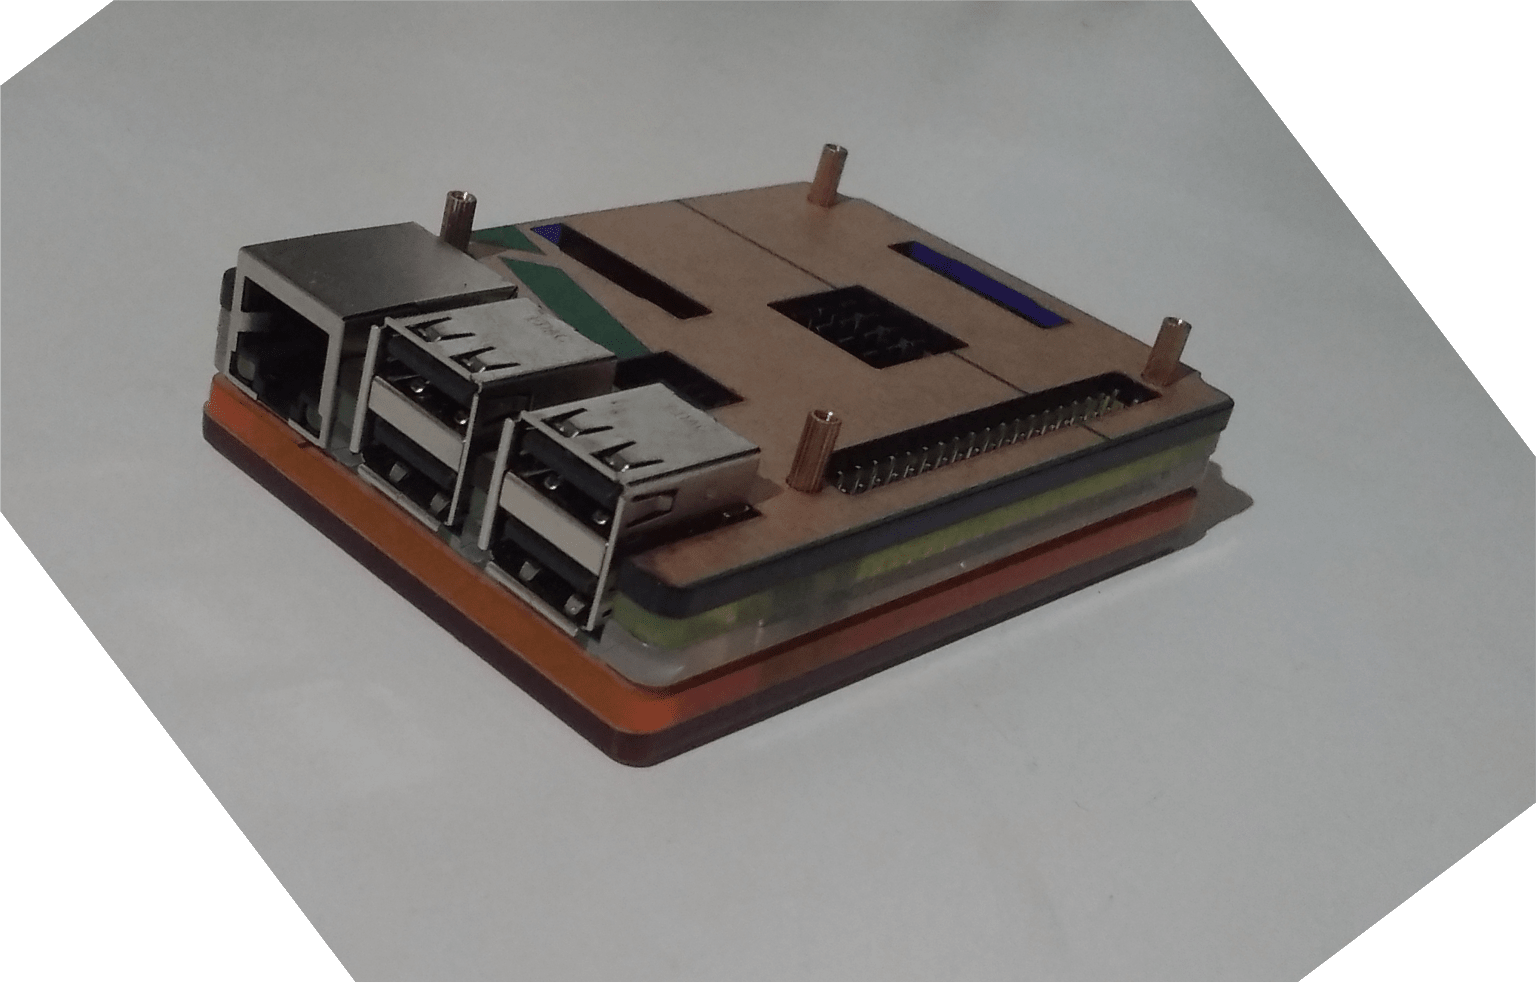
\includegraphics[scale=.20]{imagens/raspberry-min.png}}\\
\makebox[\width]{Fonte: foto tirada pelo autor} \label{Fig:raspberry_pi}
\end{figure}

O \textit{Raspberry Pi}, segundo \citeonline{oliveira}, é um computador montado em apenas uma única placa, o qual se classifica como \textit{Single-Board Computer (SBC)}. Ele ainda afirma que nesta placa, são integrados o processador, memória, portas de I/O e outros componentes que são necessários para seu funcionamento. A arquitetura presente em seu processador é um ARM, semelhantes aos processadores utilizados em celulares, tablets ou sistemas embarcados. \citeonline{richardsonwallace} afirmam que este processador é o mesmo que os encontrados no iPhone 3G e no \textit{Kindle} 2, o que permite ter uma referência sobre seu poder de processamento. De acordo com os autores, os chips ARM possuem diferentes núcleos configurados para fornecer capacidades diferentes de processamento. Seu sistema operacional padrão é uma distribuição Linux conhecida como \textit{Raspbian}, entretanto, os autores ressaltam que o usuário final não é limitado a utilizar somente este S.O. no dispositivo, ficando livre para explorar outras distribuições.

\section{COMPUTAÇÃO EM NUVEM}
De acordo com a definição da \citeonline{microsoft}, computação em nuvem é a disponibilização de diversos serviços de computação - como servidores, armazenamento, banco de dados, sistemas, entre outros serviços de TI - através da internet. A \textit{Amazon Web Service} \nocite{amazoncloudcomputing} ainda complementa que a plataforma que provê estes serviços é responsável pela manutenção de todo equipamento necessário para a disponibilização dos serviços. Tanto a \textit{Amazon Web Services (AWS)} quanto a Microsoft \textit{Azure} são plataformas conhecidas que proveem serviços de computação em nuvem.

Ambas afirmam que existem vários benefícios na utilização destes serviços. Dentre eles, uma das vantagens é relacionada ao custo, pois dispensa o gasto com qualquer tipo de equipamento para manter um datacenter local, uma vez que é utilizado uma infraestrutura já pronta e montada por estas prestadoras de serviço, que garantem a disponibilidade dos recursos através da internet \cite{amazoncloudcomputing, microsoft}.

Estes serviços são classificados em três tipos: Infraestrutura como Serviço (IaaS), Plataforma como Serviço (PaaS) e Software como Serviço (SaaS). A categoria de IaaS, segundo a definição da \citeonline{microsoft}, é a mais básica e provém toda a infraestrutura de TI, como servidores, máquinas virtuais, armazenamento, redes e sistemas operacionais. A categoria PaaS são serviços de computação que fornecem ambientes sob demanda para desenvolvimento, teste, fornecimento e gerenciamento de aplicativos de software. O SaaS fornece aplicativos de software pela nuvem sob demanda, normalmente baseadas em assinaturas.

\section{INTERNET DAS COISAS \textit{(INTERNET OF THINGS - IOT)}}
A ideia de \textit{IoT} se refere aos objetos do mundo físico gerando informações de forma autônoma para os computadores \cite{ashton}. Ele reforça que todas as informações presentes na internet foram geradas a partir de um ser humano. Uma questão pontuada por ele é referida à limitação das pessoas com relação ao tempo, atenção e precisão. Essa limitação pode resultar em ineficiência ao capturar dados sobre o mundo real. Dito isso, o autor conclui afirmando que é necessário capacitar os computadores através de seus próprios meios de coleta de informações para observarem e compreenderem o mundo físico sem a limitação da entrada de dados através de uma pessoa.

O conceito de Internet das Coisas conforme definido pelo projeto \citeonline{casagras} na introdução e idealizado por \citeonline{ashton} abordam a interconectividade e troca de informações entre os objetos do mundo físico com o mundo virtual (Figura \ref{Fig:representacao_iot}). \citeonline{dias} afirma que existem infinitas possibilidades de negócio e aplicações envolvendo o conceito de internet das coisas. Ela ainda menciona alguns nichos destes negócios, como os voltados para os bens de consumo, distribuição de energia, casas inteligentes, indústria e manufatura e transporte inteligente. Para este último nicho, a autora ainda traz algumas aplicações possíveis de serem exploradas, como notificação das condições de tráfego, controle inteligente de rotas, coordenação das rodovias e monitoramento remoto de veículos.

\begin{figure}[!ht]
\centering
\caption{Representação da interação das 'coisas' dentro do conceito de \textit{IoT}.} 
{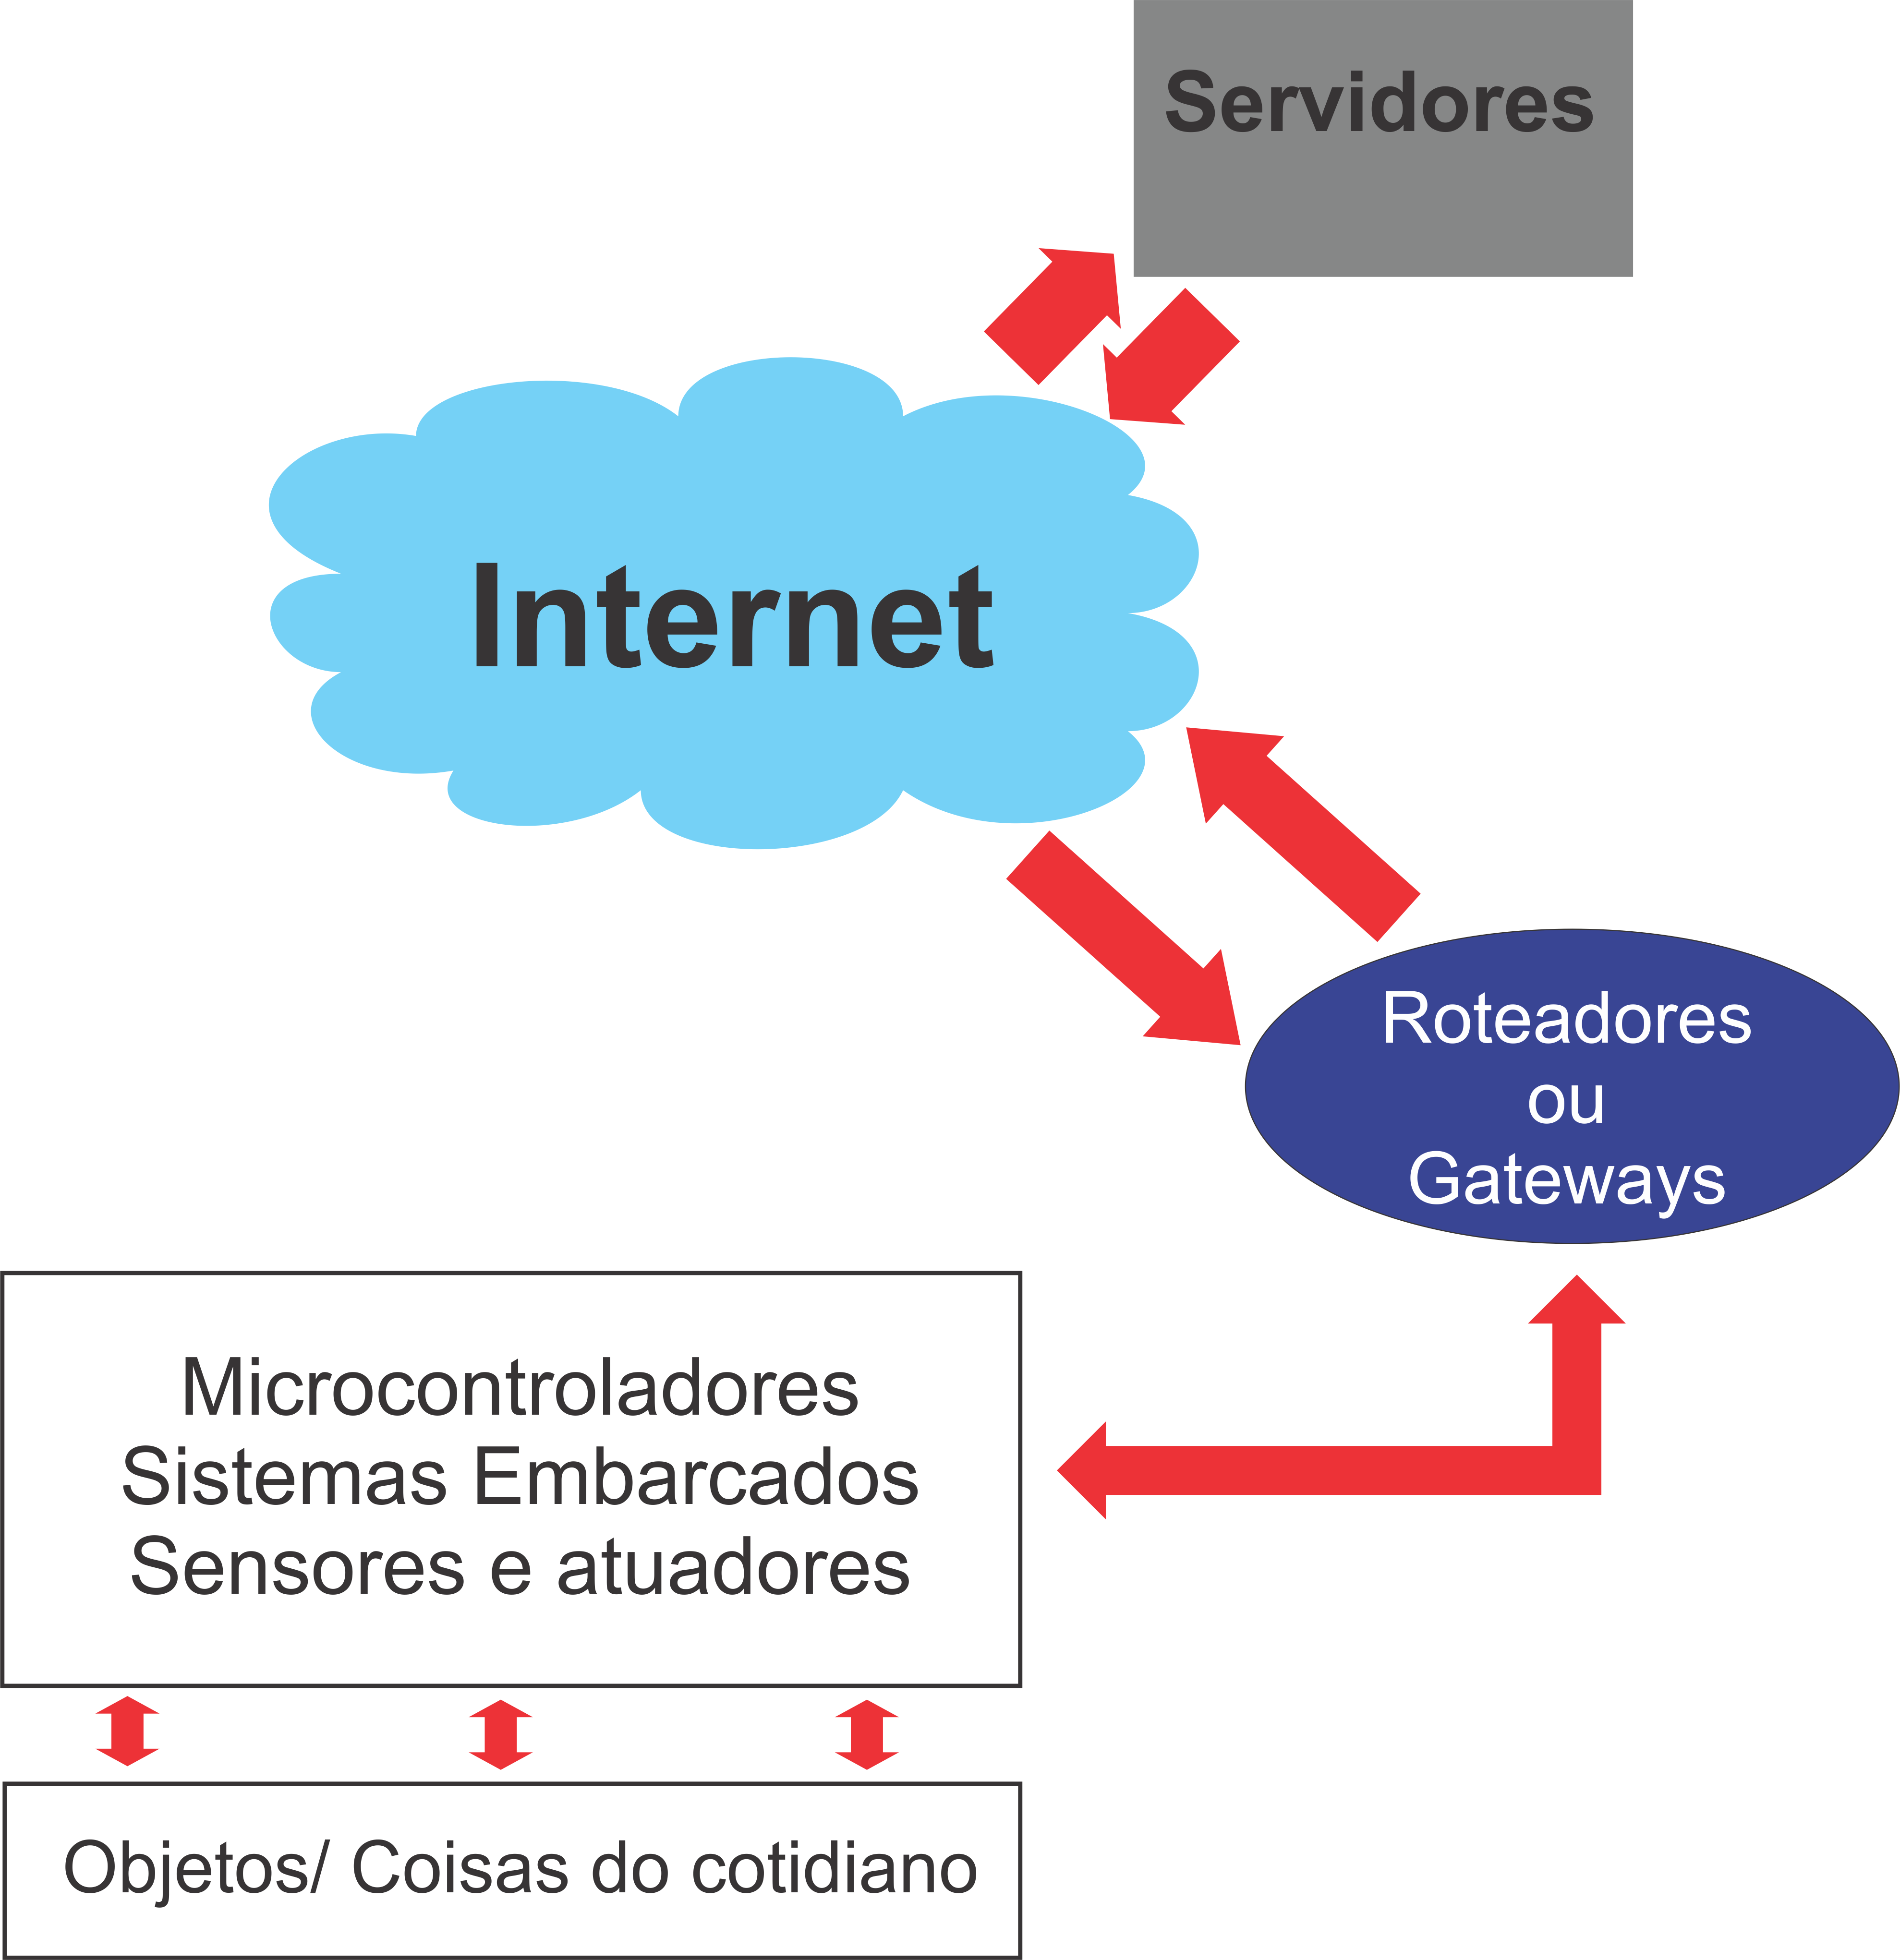
\includegraphics[scale=.40]{imagens/diagramaIOT.png}}\\
\makebox[\width]{Fonte: baseado nas obras de \citeonline{ashton}, \citeonline{casagras} e \citeonline{dias}} \label{Fig:representacao_iot}
\end{figure}

De acordo com o que foi apresentado até o momento, observam-se dois pontos importantes: primeiro, a cada evolução de um automóvel, nota-se que ele está se tornando mais informatizado e conectado; segundo, a tendência da \textit{IoT} é permitir que cada vez mais as coisas se comuniquem e troquem informações entre si, com mínima intervenção humana.
